\documentclass[10pt,twoside]{report}
\usepackage[T1]{fontenc}
\usepackage[utf8]{inputenc}
\usepackage[a4paper,margin=2.1cm,headsep=10pt]{geometry}
\usepackage{charter}
\usepackage[scaled=0.92]{helvet}
\usepackage{microtype}
\usepackage{tcolorbox}
\tcbuselibrary{skins,breakable}
\usepackage{tikz}
\usetikzlibrary{calc,shapes.geometric,positioning,arrows.meta,backgrounds,fit,decorations.pathmorphing}
\usepackage{enumitem}
\usepackage{multicol}
\usepackage{needspace}
\usepackage{titlesec}
\usepackage{fancyhdr}
\usepackage[hidelinks]{hyperref}
\usepackage{xcolor}
\usepackage{amssymb}
\usepackage{array}
\usepackage{longtable}
\usepackage{booktabs}

% ---------------------------------------------------------------- palette
\definecolor{gukdeep}{RGB}{28,54,48}     % drowned teal-green
\definecolor{gukmoss}{RGB}{92,112,74}    % moss
\definecolor{gukred}{RGB}{122,32,32}     % dried blood / dead-side
\definecolor{gukgold}{RGB}{176,141,66}   % tarnished gold
\definecolor{parch}{RGB}{243,238,224}    % parchment
\definecolor{parch2}{RGB}{247,243,232}
\definecolor{gukstone}{RGB}{74,80,78}
\definecolor{gukbone}{RGB}{223,214,192}
\definecolor{hpaper}{RGB}{236,224,197}   % handout parchment
\definecolor{hink}{RGB}{78,60,42}        % sepia ink
\definecolor{hblood}{RGB}{120,40,34}     % scrawled warnings

% ---------------------------------------------------------------- headings
\titleformat{\chapter}[display]
  {\sffamily\bfseries\color{gukdeep}}
  {\filright\sffamily\large\color{gukgold}\MakeUppercase{\chaptertitlename\ \thechapter}}
  {6pt}{\Huge\filright\scshape}
  [\vspace{2pt}{\color{gukgold}\titlerule[1.4pt]}]
\titleformat{\section}
  {\sffamily\bfseries\large\color{gukred}}{\thesection}{0.6em}{\scshape}
  [{\color{gukgold!70!black}\titlerule[0.6pt]}]
\titleformat{\subsection}
  {\sffamily\bfseries\color{gukdeep}}{\thesubsection}{0.5em}{}
\titlespacing*{\chapter}{0pt}{-18pt}{18pt}

\pagestyle{fancy}\fancyhf{}
\renewcommand{\headrulewidth}{0.4pt}
\renewcommand{\chaptermark}[1]{\markboth{\thechapter.\ #1}{}}
\fancyhead[LE]{\small\scshape\color{gukdeep}The Ruins of Guk}
\fancyhead[RO]{\small\scshape\color{gukdeep}\leftmark}
\fancyfoot[C]{\small\color{gukstone}\thepage}

% ---------------------------------------------------------------- flavor / read-aloud box
\newtcolorbox{readaloud}{
  breakable,enhanced,sharp corners,
  colback=gukdeep!7,colframe=gukdeep!55,boxrule=0.7pt,
  borderline west={3pt}{0pt}{gukgold},
  left=10pt,right=8pt,top=6pt,bottom=6pt,
  fontupper=\itshape
}

% ---------------------------------------------------------------- GM aside
\newtcolorbox{gmnote}{
  breakable,enhanced,sharp corners,
  colback=gukred!5,colframe=gukred!55,boxrule=0.6pt,
  left=8pt,right=8pt,top=4pt,bottom=4pt,
  fonttitle=\sffamily\bfseries\scshape\color{white},
  colbacktitle=gukred!80,title=Behind the Veil}

% ---------------------------------------------------------------- STAT BLOCK
\newtcolorbox{statblock}[1]{
  breakable,enhanced,sharp corners,
  colback=parch,colframe=gukred,boxrule=1pt,
  colbacktitle=gukred,coltitle=white,
  fonttitle=\sffamily\bfseries\scshape\large,
  title={#1},
  left=7pt,right=7pt,top=3pt,bottom=5pt}
\newcommand{\msub}[1]{{\itshape #1}\par}
\newcommand{\mrule}{\par\vspace{2pt}{\color{gukred}\rule{\linewidth}{1.1pt}}\par\vspace{2pt}}
\newcommand{\mthin}{\par\vspace{1pt}{\color{gukred!60}\rule{\linewidth}{0.5pt}}\par\vspace{2pt}}
\newcommand{\mfield}[2]{\noindent\textbf{\color{gukred}#1} #2\par}
\newcommand{\mhead}[1]{\par\smallskip{\sffamily\bfseries\scshape\color{gukred}#1}\par
  \vspace{-3pt}{\color{gukred}\rule{\linewidth}{0.7pt}}\par\vspace{2pt}}
\newcommand{\mtrait}[2]{\noindent\textbf{\itshape #1} #2\par\vspace{2pt}}
\newcommand{\abilities}[6]{\par\smallskip\noindent
  {\setlength{\tabcolsep}{1.5pt}%
  \begin{tabular}{@{}*{6}{p{0.15\linewidth}}@{}}
  \centering\sffamily\bfseries\color{gukred}STR &\centering\sffamily\bfseries\color{gukred}DEX
  &\centering\sffamily\bfseries\color{gukred}CON &\centering\sffamily\bfseries\color{gukred}INT
  &\centering\sffamily\bfseries\color{gukred}WIS &\centering\arraybackslash\sffamily\bfseries\color{gukred}CHA\\
  \centering #1 &\centering #2 &\centering #3 &\centering #4 &\centering #5 &\centering\arraybackslash #6\\
  \end{tabular}}\par\smallskip}

% ---------------------------------------------------------------- ITEM CARD
\newtcolorbox{itemcard}[2]{
  breakable=false,enhanced,sharp corners,
  colback=parch2,colframe=gukgold!70!black,boxrule=1pt,
  colbacktitle=gukgold!85!black,coltitle=white,
  fonttitle=\sffamily\bfseries\scshape,
  title={#1 \hfill \mdseries\upshape\footnotesize #2},
  left=7pt,right=7pt,top=3pt,bottom=5pt}
\newcommand{\itemtype}[1]{{\itshape #1}\par\vspace{2pt}{\color{gukgold!70!black}\rule{\linewidth}{0.6pt}}\par\vspace{2pt}}
\newcommand{\eqnote}[1]{\par\vspace{3pt}{\color{gukgold!70!black}\rule{\linewidth}{0.5pt}}\par
  {\footnotesize\itshape\color{gukstone}From the vaults of Norrath:~#1}\par}

% ---------------------------------------------------------------- misc
\newcommand{\dc}[1]{DC~#1}
\newcommand{\keyed}[1]{\noindent\textbf{\color{gukdeep}#1}\quad}
\setlist[itemize]{leftmargin=1.2em,itemsep=1pt,topsep=2pt}
\setlist[description]{leftmargin=0em,itemsep=2pt}
\newcommand{\roomrule}{\vspace{2pt}\hrule height 0.4pt\vspace{4pt}}

\hypersetup{pdftitle={The Ruins of Guk: A Descent in Two Ages},pdfauthor={A 5e Conversion}}

\begin{document}
\pagestyle{empty}

% ============================================================ TITLE PAGE
\begin{titlepage}
\centering
\vspace*{\fill}
\begin{tikzpicture}[remember picture,overlay]
  \fill[gukdeep] (current page.south west) rectangle (current page.north east);
  \foreach \i in {1,...,60}{
    \fill[gukmoss!\the\numexpr20+\i\relax!gukdeep,opacity=0.10]
      ($(current page.south west)+(rand*10.5+10.5,rand*7.4+7.4)$) circle (rand*0.5+0.5);}
\end{tikzpicture}
{\color{gukgold}\rule{0.7\linewidth}{1.5pt}}\par\vspace{10pt}
{\sffamily\bfseries\scshape\color{parch}\Huge The Ruins of Guk}\par\vspace{6pt}
{\sffamily\scshape\color{gukgold}\LARGE A Descent in Two Ages}\par\vspace{10pt}
{\color{gukgold}\rule{0.7\linewidth}{1.5pt}}\par\vspace{28pt}
{\itshape\color{parch}\large A drowned froglok city for Fifth Edition ---\\[2pt]
its upper warrens for heroes of the 2nd to 6th tier of life,\\[2pt]
its war-torn deeps for champions of the 13th to 17th.}\par
\vspace{40pt}
{\color{parch}\sffamily A dungeon in the tradition of the old\\ Norrathian delve beneath Innothule Swamp}\par
\vspace*{\fill}
{\footnotesize\color{gukbone}An unofficial homage. Norrath, EverQuest, and its place-names are the property of their owners; used here in loving tribute, without claim.}\par
\end{titlepage}

\clearpage
\pagestyle{fancy}
\setcounter{page}{1}
\setcounter{tocdepth}{1}
{\hypersetup{linkcolor=black}
\renewcommand{\contentsname}{\normalfont\sffamily\bfseries\scshape\color{gukdeep}The Delve, in Brief}
\tableofcontents}
\clearpage

% ============================================================ INTRO
\chapter*{On the Delving of Guk}
\addcontentsline{toc}{chapter}{On the Delving of Guk}
\markboth{On the Delving of Guk}{}

\begin{readaloud}
Innothule is a swamp that does not so much end as forget itself. Somewhere past the last stand of drowned cypress the mud firms into cut stone, and the stone descends. Frogloks built here once --- a city, and beneath the city a second city, and beneath that a war that has never been permitted to end. The swamp calls the whole of it \emph{Guk}, and does not distinguish the living from the dead, because Guk itself no longer troubles to.
\end{readaloud}

\noindent This book describes two dungeons that share one throat.

The \textbf{Upper Ruins} are a living, if wretched, place: the surviving frogloks of Guk keep a leaking township in the old market-labyrinth, trading, praying, spawning, and dying much as their grandparents did, harried by alligators, cave-spiders, restless fungus men in the mushroom farm, and troll raiders creeping up from the swamp. This is country for \textbf{4th-level characters} (a party of the 2nd to 6th level will find work here), and it is meant to be lived in as much as fought through. The frogloks are people. They have names, feuds, debts, and errands.

The \textbf{Lower Ruins} are the reason Guk is spoken of in hushed tones. Long ago the frogloks took this deep city by conquest --- and the dying curse of the people they took it from has never let them keep it in peace. Half the deep city died in a day and would not stay dead. The survivors, faithful to Mithaniel Marr, walled the living remnant into a redoubt and have held it ever since against the ghoul-kingdom that presses in from every tunnel. It is a siege with no relief and no surrender, run by a living froglok king who holds a throne first won --- and first lost --- by the hero Hoptor Thaggelum; for that same hero-king still reigns, on the other side of the wall, as the Ghoul Lord. This is country for \textbf{15th-level characters} (13th to 17th), and the war in it is real. The two sides want different things from the party, and both are right about the other.

\section*{How the Two Ages Connect}
A single flooded stair, the \emph{Long Descent}, joins the Upper Ruins to the Lower. The frogloks above know what lies below and will not go near it; a mid-level party that stumbles down the Descent unprepared is the setup for a cautionary tale, not an encounter. Run Guk as two campaigns with a decade of play between them if you like --- the same characters, older; or their students; or the town they saved, now old enough to send its own children down.

\section*{The Curse of Guk (a short history for the Game Master)}
\begin{description}
\item[The Conquest.] The frogloks came to Innothule as nomads and were revolted by the cannibal trolls who denned beneath the swamp. Under the hero-king \textbf{Hoptor Thaggelum} they stormed the trolls' ancient citadel and drove them out, taking the stone city for their own --- the city that would become Guk. The trolls they did not kill they made prisoners, and the war with the trolls of Grobb has never truly ended.
\item[The Shaman's Curse.] A single troll shaman came back for revenge. He walked into his lost city and slew frogloks with his bare hands, and when the guardsmen closed on him --- drenched to the elbows in froglok blood --- he called down the raw hatred of \textbf{Innoruuk}, the Prince of Hate. The blast killed the shaman and hundreds of froglok witnesses at a stroke, and left a curse in its wake: the souls of the froglok dead were dragged to \textbf{Innoruuk's Cauldron}, and their bodies condemned to rise and walk forever as the undead. Nearly half of Guk died that day. Among them was Hoptor Thaggelum.
\item[The Rotting.] The dead of Guk rose; then the dying; then, in the deep wards, the living who had merely despaired. Hoptor was raised by Innoruuk's power as the first and greatest ghoul --- the \textbf{Ghoul Lord} --- his court-mage rotting beside him into the \textbf{Ghoul Arch Magus, Vethyl}. Bound to the Prince of Hate, the Ghoul Lord began, and has never stopped, building an army of undead frogloks in the deep.
\item[The Wall, and the Denial.] The living survivors fled to the upper city and walled the last living wards of the deep into a redoubt, faithful to Mithaniel Marr, and there they hold still. The frogloks of the upper city --- untouched by the curse --- refuse to believe the rumor that seeps up from below: that the thing ruling the ghoul-kingdom is their own revered hero-king, subjected to so debased a torment.
\item[Upper Guk, After.] The upper city, cut off from the doomed deep, survived as a shabby remnant --- frogloks who fled the plague's edge and never went home. They are the Upper Ruins today: poor, pious, and pointedly incurious about the stair that goes down.
\end{description}

% ============================================================ GENERAL MAP
\section*{The Shape of the Whole}
\begin{center}
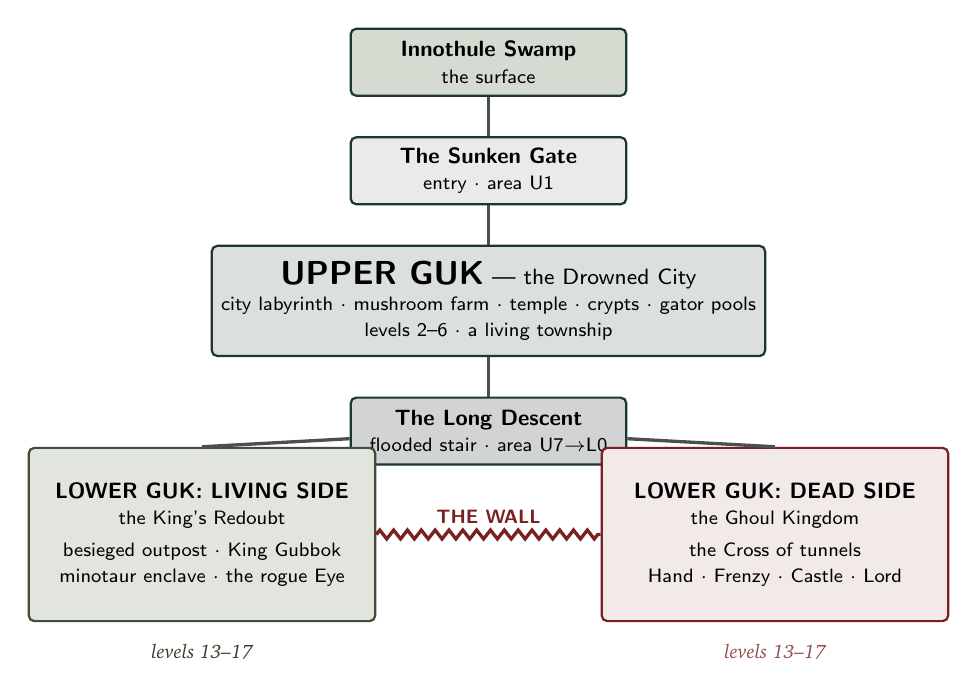
\begin{tikzpicture}[
  every node/.style={font=\sffamily\footnotesize},
  reg/.style={draw=gukdeep,fill=gukdeep!10,rounded corners=2pt,minimum width=3.5cm,minimum height=0.85cm,align=center,thick},
  deadreg/.style={draw=gukred,fill=gukred!10,rounded corners=2pt,minimum width=3.3cm,minimum height=0.8cm,align=center,thick},
  liv/.style={draw=gukmoss!70!black,fill=gukmoss!18,rounded corners=2pt,minimum width=3.3cm,minimum height=0.8cm,align=center,thick},
  link/.style={very thick,gukstone}]

\node[reg,fill=gukmoss!25] (swamp) {\textbf{Innothule Swamp}\\{\scriptsize the surface}};
\node[reg,below=0.5cm of swamp] (gate) {\textbf{The Sunken Gate}\\{\scriptsize entry $\cdot$ area U1}};
\node[reg,below=0.5cm of gate,minimum width=6.2cm,minimum height=1.4cm,fill=gukdeep!16] (upper)
  {\textbf{\large UPPER GUK} --- the Drowned City\\{\scriptsize city labyrinth $\cdot$ mushroom farm $\cdot$ temple $\cdot$ crypts $\cdot$ gator pools}\\{\scriptsize levels 2--6 $\cdot$ a living township}};
\node[reg,below=0.5cm of upper,fill=gukstone!25] (descent) {\textbf{The Long Descent}\\{\scriptsize flooded stair $\cdot$ area U7$\to$L0}};

\draw[link] (swamp)--(gate); \draw[link](gate)--(upper); \draw[link](upper)--(descent);

% lower split
\node[below=0.75cm of descent] (splitanchor) {};
\node[liv,left=1.3cm of splitanchor,minimum width=4.4cm,minimum height=2.2cm,align=center] (living)
  {\textbf{LOWER GUK: LIVING SIDE}\\{\scriptsize the King's Redoubt}\\[2pt]{\scriptsize besieged outpost $\cdot$ King Gubbok}\\{\scriptsize minotaur enclave $\cdot$ the rogue Eye}};
\node[deadreg,right=1.3cm of splitanchor,minimum width=4.4cm,minimum height=2.2cm,align=center] (dead)
  {\textbf{LOWER GUK: DEAD SIDE}\\{\scriptsize the Ghoul Kingdom}\\[2pt]{\scriptsize the Cross of tunnels}\\{\scriptsize Hand $\cdot$ Frenzy $\cdot$ Castle $\cdot$ Lord}};

\draw[link] (descent)-- (living.north);
\draw[link] (descent)-- (dead.north);
\draw[very thick,gukred,decorate,decoration={zigzag,segment length=5pt,amplitude=1.6pt}]
  (living.east)--(dead.west) node[midway,above,font=\scriptsize\sffamily\bfseries,text=gukred]{THE WALL};
\node[below=0.15cm of living,font=\scriptsize\itshape,text=gukmoss!60!black]{levels 13--17};
\node[below=0.15cm of dead,font=\scriptsize\itshape,text=gukred!80]{levels 13--17};
\end{tikzpicture}
\end{center}

\noindent The maps that open each half of the book are schematic --- corridors are drawn as lines, not to scale --- and every keyed area carries a technical description (dimensions, light, hazards) in the appendix. Run the geography loosely; Guk is meant to feel like a place people got lost in.

\clearpage

% ####################################################################
\chapter{Upper Guk --- The Drowned City}
% ####################################################################
\begin{readaloud}
The gate lets you out onto a gallery above the old market, and for a moment you mistake the sound for rain. It is not rain. It is Guk: ten thousand drips from a ceiling that has wept for a century, the wet slap of froglok feet on green stone, the croak-and-answer of a people who have made a home of a ruin because the ruin is all they were left. Somewhere a smith is working. Somewhere a child is crying. Somewhere, far down, something old turns over in its sleep.
\end{readaloud}

\noindent Upper Guk is a \emph{town} that happens to be a dungeon. The frogloks here are the great-grandchildren of refugees, and they have built ordinary lives in a place of extraordinary decay: markets in the labyrinth, a temple to Mithaniel Marr kept lit against the dark below, spawning-pools jealously guarded, and a wary peace with the fungus-folk who share their walls. Threats are local and legible --- a gator taking swimmers, a spider-brood in the granary, trolls at the swamp-gate, the mushroom farm gone strange. \textbf{Treat the townsfolk as quest-givers and neighbors first, and monsters second.} A party that murders its way through the market will find every door in Guk shut to it.

\section{Map of the Upper Ruins}
\begin{center}
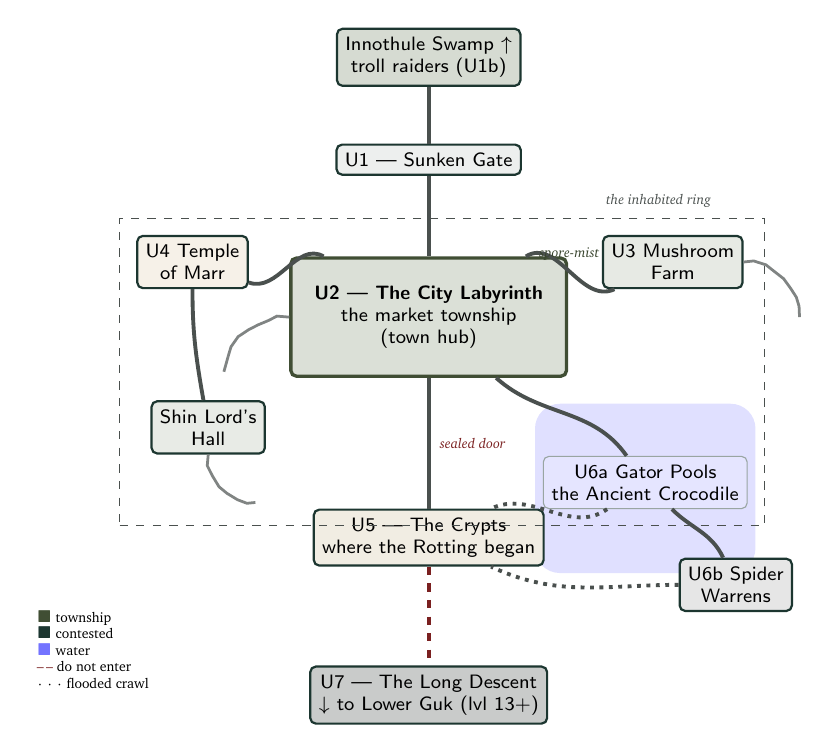
\begin{tikzpicture}[
  font=\sffamily\scriptsize,
  room/.style={draw=gukdeep,fill=gukdeep!8,rounded corners=2pt,align=center,thick,inner sep=3pt},
  town/.style={draw=gukmoss!70!black,fill=gukmoss!22,rounded corners=2pt,align=center,very thick,inner sep=3pt},
  tun/.style={gukstone,line width=1.4pt},
  wet/.style={draw=gukdeep!45,fill=blue!10,rounded corners=2pt,align=center,inner sep=3pt},
  stub/.style={gukstone!70,line width=1pt,decorate,decoration={random steps,segment length=4pt,amplitude=0.5pt}}]

% water pool behind the gator pools
\fill[blue!12,rounded corners=9pt] (6.35,5.85) rectangle (9.15,8.0);

\node[room,fill=gukmoss!25] (swamp) at (5,12.4) {Innothule Swamp $\uparrow$\\{\scriptsize troll raiders (U1b)}};
\node[room] (u1) at (5,11.1) {U1 --- Sunken Gate};
\node[town,minimum width=3.5cm,minimum height=1.5cm] (u2) at (5,9.1) {\textbf{U2 --- The City Labyrinth}\\{\scriptsize the market township}\\{\scriptsize (town hub)}};
\node[room,fill=gukgold!12] (u4) at (2.0,9.8) {U4 Temple\\of Marr};
\node[room,fill=gukmoss!14] (shin) at (2.2,7.7) {Shin Lord's\\Hall};
\node[room,fill=gukmoss!15] (u3) at (8.1,9.8) {U3 Mushroom\\Farm};
\node[wet] (u6a) at (7.75,7.0) {U6a Gator Pools\\{\scriptsize the Ancient Crocodile}};
\node[room,fill=gukstone!14] (u6b) at (8.9,5.7) {U6b Spider\\Warrens};
\node[room,fill=gukbone!45] (u5) at (5,6.3) {U5 --- The Crypts\\{\scriptsize where the Rotting began}};
\node[room,fill=gukstone!30] (u7) at (5,4.3) {U7 --- The Long Descent\\{\scriptsize $\downarrow$ to Lower Guk (lvl 13+)}};

\draw[tun] (swamp)--(u1);
\draw[tun] (u1) to[out=-90,in=90] (u2);
\draw[tun] (u2) to[out=150,in=-20] (u4);
\draw[tun] (u4) to[out=-90,in=100] (shin);
\draw[tun] (u2) to[out=32,in=205] node[midway,above,font=\tiny\itshape,text=gukmoss!60!black]{spore-mist}(u3);
\draw[tun] (u2) to[out=-42,in=125] (u6a);
\draw[tun] (u6a) to[out=-45,in=115] (u6b);
\draw[tun] (u2) to[out=-90,in=90] node[midway,right,font=\tiny\itshape,text=gukred]{sealed door}(u5);
\draw[tun,gukred,dashed] (u5)--(u7);
\draw[tun,dotted] (u6a) to[out=-145,in=25] (u5);
\draw[tun,dotted] (u6b) to[out=180,in=-25] (u5);
\draw[stub] (u2.west) to[out=180,in=90] ++(-0.8,-0.7);
\draw[stub] (u3.east) to[out=0,in=90] ++(0.7,-0.7);
\draw[stub] (shin.south) to[out=-90,in=180] ++(0.6,-0.6);

\node[draw=gukstone,dashed,inner sep=6pt,fit=(u4)(u3)(u6a)(u2)(shin),
  label={[font=\tiny\itshape,text=gukstone]above right:the inhabited ring}] {};

\node[font=\tiny,align=left,anchor=north west] at (-0.1,5.5) {\begin{tabular}{@{}l@{}}
\textcolor{gukmoss!70!black}{$\blacksquare$}~township\\
\textcolor{gukdeep}{$\blacksquare$}~contested\\
\textcolor{blue!55}{$\blacksquare$}~water\\
\textcolor{gukred}{--\,--}~do not enter\\
$\cdots$~flooded crawl\end{tabular}};
\end{tikzpicture}
\end{center}

% ------------------------------------------------------------------
\section{U1 --- The Sunken Gate}
\begin{readaloud}
A froglok in a patched tabard leans on a hooked spear at the gate, watching you come with the flat, unbothered patience of someone who has seen adventurers before and buried most of them. ``Dry-skins,'' he says, not unkindly. ``Down from the swamp. You'll want the market, then. Keep your hands where a body can see them and don't feed the fungus.''
\end{readaloud}
The Sunken Gate is a checkpoint gallery overlooking U2, manned in shifts by the town watch. It is the party's introduction to the idea that Guk has \emph{rules}. The gate-warden, \textbf{Sergeant Ploomb} (use \emph{Froglok Sentry}), will let armed strangers pass but marks them; if the party later causes trouble, the watch already has their number.

\subsection*{U1b --- The Troll Stair (the swamp door)}
A side-passage from the gate climbs toward Innothule. Twice a tenday, troll raiders from the swamp clans creep up it to steal spawnlings and stores. This is the town's most reliable low-stakes threat and the hook for the \emph{Hold the Stair} quest below.

% ------------------------------------------------------------------
\section{U2 --- The City Labyrinth (the township)}
\begin{readaloud}
The market fills the shell of what must once have been a grand concourse: a maze of stalls roofed in stretched gator-hide, lit by cold green fungus-lanterns and the occasional stolen torch. Frogloks haggle in wet clicking speech over dried fish, swamp-iron, and charms against the deep. Everywhere the stone remembers a finer city --- a carved frieze here, a drowned fountain there --- and everywhere the frogloks have simply built over it, the way lichen builds over a grave.
\end{readaloud}

This is the \textbf{town hub}: safe by default, full of errands, and the emotional center of the Upper Ruins. Run it as a settlement. The frogloks are proud, poor, devout, and funny; they croak-laugh at their own dark jokes and treat outsiders as weather --- to be endured and occasionally profited from.

\subsection*{Notable Folk of the Labyrinth}
\begin{description}
\item[Elder Nurga, the Marr-Speaker] (\emph{Froglok Shaman}). Ancient, half-blind, and the closest thing Guk has to a mayor. She remembers her grandmother's stories of the deep city and is the only townsperson who will speak plainly about what is down the sealed stair. She is the party's chief employer and moral compass. \emph{Quest-giver: The Crypt-Seal; The Long Descent (warning, not invitation).}
\item[The Froglok Shin Lord] (\emph{stat block; a paladin}). One of the last of the ancient froglok paladin order, and the true authority in Upper Guk --- the Shin clan holds the upper city, and he holds the Shin. He defends the halls against both the troll menace and the undead that seep up from the low ruins, and he bears the holy blade \textbf{Ghoulbane} (item card). Weary in a way sleep doesn't fix, he hires the party for the troll problem and, if they prove reliable, for the far worse thing below. \emph{Quest-giver: Hold the Stair; The Granary.}
\item[Old Grubb the Gatorhand] (\emph{Froglok Sentry}, missing three fingers). Guk's hunter and its worst gambler. He owes everyone and knows the gator pools better than anyone alive. \emph{Quest-giver: The Restless God (the Ancient Crocodile).}
\item[Spore-Speaker Uth] --- \emph{not a froglok}. A fungus-man emissary permitted, uneasily, to keep a stall of medicinal fungus at the market's edge (see U3). Uth speaks in a chorus of soft pops and a borrowed, formal Common. It is the town's physician and its greatest source of unease. \emph{Quest-giver: The Farm Sickens.}
\item[Little Krik] (\emph{Froglok Spawnling}, a child). Underfoot, fearless, forever losing things down holes no adult can fit into. A source of rumor, comic relief, and --- once --- of the party learning something is very wrong before the adults will admit it.
\end{description}

\subsection*{Rumors at the Stalls (roll or choose)}
\begin{enumerate}[leftmargin=1.6em,itemsep=1pt]
\item ``The gators are bolder this season. Grubb says something in the deep pool is \emph{driving} them up.''
\item ``Uth's kind have gone quiet in their farm. The mist smells wrong --- sweet, like rot pretending to be flowers.''
\item ``Trolls took two spawnlings off the stair last tenday. the Shin Lord's knights are stretched thin.''
\item ``Elder Nurga hasn't slept. She keeps standing at the sealed door like she's listening for something to knock.''
\item ``There's a crack in the crypt seal. Little Krik swears he heard singing down there. Krik swears a lot of things.''
\end{enumerate}

% ------------------------------------------------------------------
\section{U3 --- The Mushroom Farm (the Fungus Warren)}
\begin{readaloud}
Past a curtain of hanging root the air goes warm and thick and faintly luminous. Shelf-fungus climbs the walls in slow terraces; puffballs the size of shields exhale glowing spores that drift and settle and drift again. In the center of the farm stands the Fungus Ancient itself --- a fungus man the size of an oak, ringed by lesser fungus-folk who sway to a rhythm you cannot hear. When it speaks, the whole farm pops and sighs the words a half-beat behind, an echo of an echo.
\end{readaloud}

The fungus men of Guk are old residents --- older, perhaps, than the frogloks --- and until lately they have been quiet neighbors, trading medicine and light for salt and being left alone. Something has changed. Their eldest, the \textbf{Fungus Ancient}, has fallen into a strange fever, and its spore-song has begun to turn its own children feral and to seep, sweetly, toward the town.

\begin{gmnote}
The truth (for the \emph{Farm Sickens} quest): the rot creeping up from Lower Guk --- the same necrotic taint the Archmagus works far below --- has reached the fungal network's deepest roots. The Fungus Ancient is not malicious; it is \emph{sick}, and its sickness is the first faint tide-mark of the deep war rising. Curing it (a ritual, a rare reagent from the crypts, or simply severing the tainted root) is a genuine choice with genuine costs. Burning the farm is faster and turns a future ally into a graveyard.
\end{gmnote}

% ------------------------------------------------------------------
\section{U4 --- The Temple of Marr}
\begin{readaloud}
Someone keeps this place. Amid all of Guk's damp decay the little temple is scrubbed, its brazier fed, its silver Idol of the Truthbringer polished to catch what light there is. Mithaniel Marr, god of valor, stands in worn relief above the altar with his hand outstretched --- the same gesture, the priests say, with which he once saved the deep city and told it only to hold.
\end{readaloud}
The temple is Guk's heart and its rest-point: a place of healing, sanctuary, and the town's memory of who it was before it was a ruin. \textbf{Sister Vellka} (\emph{Froglok Shaman}) tends it and will restore, bless, and shelter the party --- and, if they earn it, entrust to them the \emph{Testament of the Marr}, a relic that matters enormously in the deep war to come (see item cards). The temple is also where a party learns \emph{why} the frogloks hold: not from strength, but from a promise.

% ------------------------------------------------------------------
\section{U5 --- The Crypts}
\begin{readaloud}
The sealed door groans open on cold that has nothing to do with the swamp. Here the old frogloks laid their dead in wall-niches, generation on generation, and here --- the histories agree --- the Rotting first showed itself, a century ago, when a body that should have lain still sat up. The seal has held since. The seal is cracked now. From somewhere below the niches, faint and patient, comes a sound like a lullaby sung with too many voices.
\end{readaloud}
The Crypts are the tonal hinge of Upper Guk: the point where the friendly township brushes against the horror beneath it. For a mid-level party this is a hard, eerie delve --- skeletal dead, a lone escaped ghoul, spore-blighted corpses where the fungus taint has met the crypt --- but \textbf{not} the deep war itself. The lullaby is bait. Follow it and you find the head of the Long Descent (U7), and a wrongness rising up it that a wise party will report to Elder Nurga and then leave well alone until they are far stronger.

\begin{gmnote}
The Crypts are the seam between the two ``ages'' of the adventure. A 4th-level party should be able to reseal the crypt (a skill challenge / short ritual) and \emph{choose not to go down}. If your table insists on descending, they die instructively --- or, if you are running one continuous campaign, this is where you time-skip and bring them back at 13th+.
\end{gmnote}

% ------------------------------------------------------------------
\section{U6 --- The Gator Pools \& Spider Warrens}
\subsection*{U6a --- The Gator Pools}
A chain of flooded chambers where the frogloks farm fish and the crocodiles farm frogloks. In the deepest, oldest pool lives the \textbf{Ancient Crocodile} --- a monstrous reptile said to have denned here since long before the frogloks came, older than Guk itself. It is not evil and takes no side; it is simply \emph{old}, and vast, and hungry on its own schedule. The frogloks revere it as an earth-god of the swamp and will not raise a hand against it, and its recent restlessness (see rumors) has them badly frightened --- for when the swamp's oldest thing grows uneasy, something deep is wrong. A superb set-piece: dark water, a hunter's guide who talks too much, and a god that fights on \emph{its} terms.
\subsection*{U6b --- The Spider Warrens}
The town granary backs onto a warren of cave-spiders that periodically boils over into the stores. Cramped, webbed, and claustrophobic --- a good showcase for a party that has learned to use Guk's terrain. The brood-mother is a named threat (\emph{Giant Cave Spider}, scaled up).

% ------------------------------------------------------------------
\section{Upper Guk Quest Lines}
Each quest is seeded in the township and pays in coin, goodwill, and access.

\subsection*{Hold the Stair (the Shin Lord)}
Trolls raid the swamp-gate (U1b). A tiered quest: repel a raid (combat), then track the raiders to a swamp-side camp, then \emph{decide} --- the trolls are starving, driven up by something worse in the swamp, and the Shin Lord would rather have a truce than a war he can't win. Diplomacy or steel; the town remembers which.
\subsection*{The Restless God (Grubb)}
The \textbf{Ancient Crocodile} of U6a has grown restless, and Grubb (who half-worships and wholly fears it) begs the party to learn why before it takes more swimmers. The quest is deliberately a moral fork: \emph{appease} the god (a rite, an offering, learning that its unease is the deep curse rising --- a genuine omen of Lower Guk), or, sacrilegiously, \emph{slay} it for the fabled \textbf{Gatorscale} hide (item card) and earn the frogloks' lasting disgust. Either way, Grubb's undying, financially ruinous loyalty.
\subsection*{The Farm Sickens (Uth / Nurga)}
Investigate the sickening mushroom farm (U3). Leads, if pursued, to the crypt-taint (U5) and the first hint of the deep war. The party's choice here --- cure or cull --- determines whether the fungus men are an ally or a scar in any later deep campaign.
\subsection*{The Crypt-Seal (Nurga)}
Reseal the cracked crypt (U5) before the lullaby draws more of the town's curious down it. The capstone of the Upper Ruins: a haunted delve, a moral test (a trapped, pitiable escaped ghoul that was once a person), and the door, firmly shut, on the age to come.

\clearpage

% ####################################################################
\chapter{Lower Guk --- The War That Never Ended}
% ####################################################################
\begin{readaloud}
The Long Descent ends in water to the knee and a smell you will not forget: cold rot, wet iron, and old incense burning against both. Ahead the tunnel forks. To one side a horn sounds --- a living horn, froglok throats on a wall, challenging you. To the other, nothing answers, which is worse. This is the deep city, and it has been at war with itself for a hundred years without an hour's ceasefire. You have arrived in the middle of it, and both sides have already seen you.
\end{readaloud}

\noindent Lower Guk is two dungeons divided by one wall. The \textbf{Living Side} is a besieged froglok outpost --- disciplined, desperate, ruled by a king who has never known peace. The \textbf{Dead Side} is a ghoul kingdom laid out as a great cross of tunnels, ruled by that king's own cursed ancestor. Between them runs the Wall, held by valor and a god's old promise.

This half of the adventure is built for \textbf{13th- to 17th-level characters} and for \emph{choices}. The living want the party to break the siege; the minotaurs want a price; the dead want the party's death and, some of them, its help. Nearly everyone in Lower Guk is lying about something, and the war is real enough that the party's decisions move the front.

\section{Map of the Lower Ruins}
\begin{center}
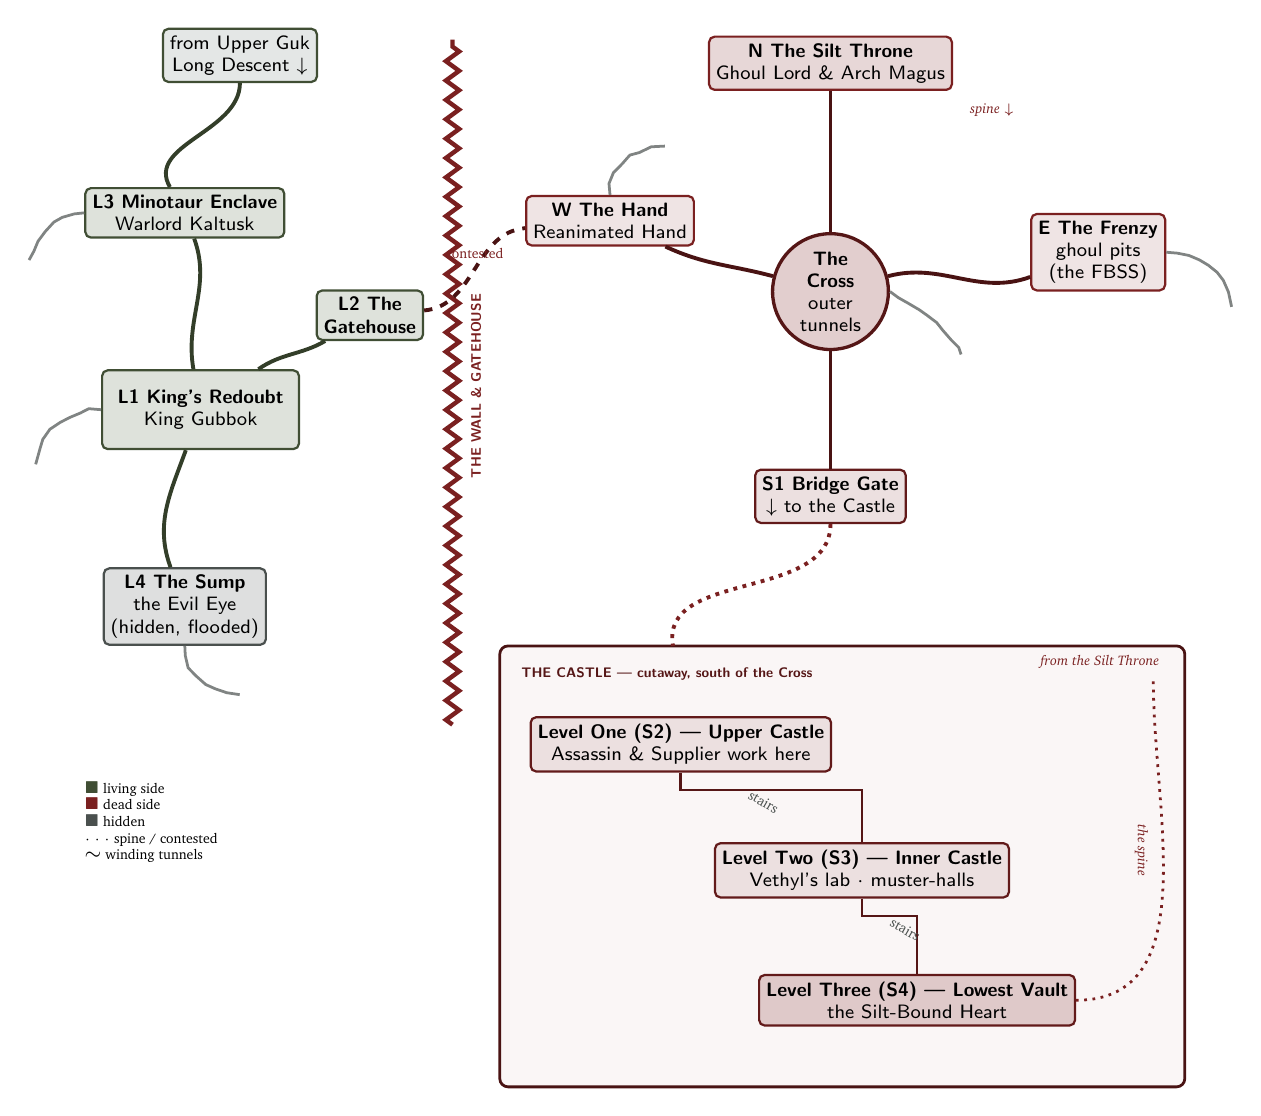
\begin{tikzpicture}[
  font=\sffamily\scriptsize,
  liv/.style={draw=gukmoss!70!black,fill=gukmoss!20,rounded corners=2pt,align=center,thick,inner sep=2.5pt},
  dead/.style={draw=gukred,fill=gukred!12,rounded corners=2pt,align=center,thick,inner sep=2.5pt},
  hub/.style={draw=gukred!70!black,fill=gukred!22,align=center,very thick,inner sep=2pt,circle},
  cast/.style={draw=gukred!80!black,fill=gukred!14,rounded corners=2pt,align=center,thick,inner sep=2.5pt},
  livtun/.style={gukmoss!55!black,line width=1.4pt},
  deadtun/.style={gukred!60!black,line width=1.4pt},
  stub/.style={gukstone!70,line width=1pt,decorate,decoration={random steps,segment length=4pt,amplitude=0.5pt}}]

% ================= THE WALL =================
\draw[gukred,line width=1.6pt,decorate,decoration={zigzag,segment length=7pt,amplitude=2.4pt}]
   (4.9,4.6)--(4.9,13.3);
\node[rotate=90,font=\tiny\sffamily\bfseries,text=gukred] at (5.2,8.9){THE WALL \& GATEHOUSE};

% ================= LIVING SIDE (west) =================
\node[liv,fill=gukdeep!12] (descent) at (2.2,13.1) {from Upper Guk\\{\scriptsize Long Descent }$\downarrow$};
\node[liv] (mino) at (1.5,11.1) {\textbf{L3 Minotaur Enclave}\\{\scriptsize Warlord Kaltusk}};
\node[liv,minimum width=2.5cm,minimum height=1.0cm] (redoubt) at (1.7,8.6) {\textbf{L1 King's Redoubt}\\{\scriptsize King Gubbok}};
\node[liv] (wallg) at (3.85,9.8) {\textbf{L2 The}\\\textbf{Gatehouse}};
\node[liv,fill=gukstone!18,draw=gukstone] (sump) at (1.5,6.1) {\textbf{L4 The Sump}\\{\scriptsize the Evil Eye}\\{\scriptsize (hidden, flooded)}};

\draw[livtun] (descent) to[out=-90,in=120] (mino);
\draw[livtun] (mino) to[out=-70,in=100] (redoubt);
\draw[livtun] (redoubt) to[out=35,in=-150] (wallg);
\draw[livtun] (redoubt) to[out=-110,in=110] (sump);
\draw[stub] (redoubt.west) to[out=180,in=90] ++(-0.8,-0.7);
\draw[stub] (mino.west) to[out=180,in=60] ++(-0.7,-0.6);
\draw[stub] (sump.south) to[out=-90,in=180] ++(0.7,-0.6);

% ================= DEAD SIDE (east) =================
\node[dead] (hand) at (6.9,11.0) {\textbf{W The Hand}\\{\scriptsize Reanimated Hand}};
\node[hub] (cross) at (9.7,10.1) {\textbf{The}\\\textbf{Cross}\\{\scriptsize outer}\\{\scriptsize tunnels}};
\node[dead,fill=gukred!18] (throne) at (9.7,13.0) {\textbf{N The Silt Throne}\\{\scriptsize Ghoul Lord \& Arch Magus}};
\node[dead] (frenzy) at (13.1,10.6) {\textbf{E The Frenzy}\\{\scriptsize ghoul pits}\\{\scriptsize (the FBSS)}};
\node[cast] (bridge) at (9.7,7.5) {\textbf{S1 Bridge Gate}\\{\scriptsize $\downarrow$ to the Castle}};

\draw[deadtun,dashed] (wallg) to[out=5,in=185] node[midway,above,font=\tiny,text=gukred]{contested} (hand);
\draw[deadtun] (hand) to[out=-25,in=165] (cross);
\draw[deadtun] (cross) to[out=90,in=-90] (throne);
\draw[deadtun] (cross) to[out=15,in=200] (frenzy);
\draw[deadtun] (cross) to[out=-90,in=90] (bridge);
\draw[stub] (frenzy.east) to[out=0,in=90] ++(0.8,-0.7);
\draw[stub] (hand.north) to[out=90,in=180] ++(0.7,0.6);
\draw[stub] (cross.east) to[out=-35,in=120] ++(0.9,-0.8);
\node[font=\tiny\itshape,text=gukred,anchor=west] at (11.35,12.4) {spine $\downarrow$};

% ================= CASTLE CUTAWAY =================
\begin{scope}[shift={(5.5,0)}]
  \draw[draw=gukred!60!black,line width=1pt,fill=gukred!4,rounded corners=3pt] (0,0) rectangle (8.7,5.6);
  \node[font=\tiny\sffamily\bfseries,text=gukred!70!black,anchor=north west] at (0.15,5.45)
     {THE CASTLE --- cutaway, south of the Cross};
  \node[cast,minimum width=3.3cm] (l1) at (2.3,4.35) {\textbf{Level One (S2) --- Upper Castle}\\{\scriptsize Assassin \& Supplier work here}};
  \node[cast,minimum width=3.7cm] (l2) at (4.6,2.75) {\textbf{Level Two (S3) --- Inner Castle}\\{\scriptsize Vethyl's lab $\cdot$ muster-halls}};
  \node[cast,minimum width=4.0cm,fill=gukred!24] (l3) at (5.3,1.1) {\textbf{Level Three (S4) --- Lowest Vault}\\{\scriptsize the Silt-Bound Heart}};
  \draw[gukred!70!black,line width=1pt] (l1.south)--++(0,-0.22)-|(l2.north);
  \draw[gukred!70!black,line width=1pt] (l2.south)--++(0,-0.22)-|(l3.north);
  \node[font=\tiny,text=gukstone,rotate=-30] at (3.35,3.62){stairs};
  \node[font=\tiny,text=gukstone,rotate=-30] at (5.15,2.0){stairs};
  % spine down the right wall, from the throne above
  \draw[gukred,dotted,line width=1pt] (8.3,5.15) to[out=-90,in=0] (l3.east);
  \node[font=\tiny\itshape,text=gukred,anchor=east] at (8.5,5.4){from the Silt Throne};
  \node[font=\tiny\itshape,text=gukred,rotate=-90] at (8.15,3.0){the spine};
\end{scope}
\draw[deadtun,dotted,gukred] (bridge.south) to[out=-90,in=100] (7.7,5.6);

% ================= LEGEND =================
\node[font=\tiny,align=left,anchor=north west] at (0.1,4.0) {\begin{tabular}{@{}l@{}}
\textcolor{gukmoss!70!black}{$\blacksquare$}~living side\\
\textcolor{gukred}{$\blacksquare$}~dead side\\
\textcolor{gukstone}{$\blacksquare$}~hidden\\
$\cdots$~spine / contested\\
{\scriptsize$\sim$}~winding tunnels\end{tabular}};
\end{tikzpicture}
\end{center}
\noindent The dead side is a \textbf{cross} of winding tunnels: a central crossroads (the Outer Tunnels) with the Hand to the west, the Frenzy to the east, and the Silt Throne to the north. To the south the Bridge Gate opens onto the \textbf{Castle}, which descends through three levels --- Upper Castle, Inner Castle, and the Lowest Vault (see the cutaway on the map). A ``spine'' passage links the Silt Throne directly to the Vault, behind the front, so the Ghoul Lord's court can move troops and reach the phylactery without crossing the open Cross. The living side hangs off the Wall to the west --- the Redoubt, the Minotaur Enclave above it, and, in the flooded Sump below, a secret that is eating the defense from within.

% ==================================================================
\section{The Living Side --- The King's Redoubt}
\begin{readaloud}
They let you through a murder-hole gate under the eyes of a dozen crossbows, and then, absurdly, they cheer --- because you are alive, and new, and in Guk that is enough to be glad of. The Redoubt is a fortress made of a palace's bones: throne-room turned command-post, ballroom turned barracks, every window a firing-slit, every wall scrawled with the tally-marks of a siege that stopped being counted decades ago. On a camp-stool where a throne should be sits a froglok in dented Marr-silver, older than his years, who looks at you the way a drowning man looks at driftwood.
\end{readaloud}

\subsection*{L1 --- The Redoubt \& the King}
\textbf{The Froglok King, Gubbok the Undrowned} (\emph{stat block, back of book}) is the living heart of Lower Guk: a paladin-king of Marr, valiant, exhausted, and privately certain the war is being lost by inches. He holds the throne first raised by the hero Hoptor Thaggelum, and he is a \emph{good} king in a hopeless post. He wants three things, in order: to hold the Wall, to break the siege, and --- though he will not say it first --- to grant final rest to the founder of his own crown, the hero-king now reigning across the wall as the Ghoul Lord. The party is the first real hope he has had in years, and he knows better than to trust hope.

\begin{gmnote}
\textbf{The symmetry to play.} King Gubbok holds the throne first won by \textbf{Hoptor Thaggelum} --- the hero-king who conquered Guk from the trolls and died in the Shaman's Curse. That same Hoptor now reigns across the wall as the Ghoul Lord, raised by Innoruuk. Gubbok half-knows this and cannot bear to say it aloud; the frogloks of the upper city deny it outright. It is the private horror of his reign that the thing besieging him is the founder of his own crown, and that ending the siege means ending Guk's greatest hero a second time. Do not state this baldly; let the party discover it, and let it cost Gubbok something when they do.
\end{gmnote}

\subsection*{L2 --- The Wall \& Gatehouse}
The fortified frontier itself: a Marr-blessed rampart across the mouth of the deep city, held in shifts by the \emph{Froglok Royal Guard}. The Wall has not moved in a century --- not because the living are winning, but because a promise holds it. \textbf{Sister Vellka's Testament} (if the party carried it down from Upper Guk) can renew that blessing; without renewal, the Wall is quietly failing, and the GM should let the party feel it (guards whispering that the stone ``feels thinner'' at night).

\subsection*{L3 --- The Minotaur Enclave (the politics)}
\begin{readaloud}
Above the Redoubt, behind a barricade of their own making, the minotaurs keep their hall --- refugees from some older war, bull-headed and iron-proud, neither froglok nor ghoul and trusting neither. Their warlord fills a doorway, an axe across his shoulders that two frogloks could not lift, and he regards you down the length of his snout with the weariness of a creature who has been asked to pick a side too many times.
\end{readaloud}
\textbf{Warlord Kaltusk of the Underhorn} (\emph{Minotaur Lord}, stat block) leads a clan of minotaurs who hold the high ground above the Redoubt. Minotaurs are old residents of Guk's living side --- elders, patriarchs, and greater minotaurs have denned in these halls as long as the frogloks have --- and they are not the king's subjects but his uneasy tenants, bound by an old, fraying treaty. The minotaurs are strong enough to break the siege \emph{or} to doom the Wall --- and Kaltusk is weighing which serves his people. \textbf{This is the living side's great political quest:} the party must secure the minotaur alliance (honor an old debt, win a rite of single combat, expose who has been poisoning the treaty --- see the Eye, below) or watch the front collapse when the minotaurs withdraw.

\subsection*{L4 --- The Sump \& the Evil Eye (the saboteur)}
\begin{readaloud}
The lowest, wettest ward of the Redoubt is a flooded sump the guards avoid, ``on account of the bad air.'' The bad air has an eye. Ten of them. Something floats in the dark over the black water --- a bloated orb ringed with writhing stalks, each ending in a small malignant star --- and it has been down here a long time, whispering up through the pipes into the dreams of a besieged garrison, turning ally against ally, one poisoned word at a time.
\end{readaloud}
\textbf{The Evil Eye of Guk} --- which the living have come to call \textbf{Ythocc} (\emph{stat block}) --- is a lone \emph{evil eye}, a lesser cousin of the beholders, washed up in Guk's underworks from some deeper delve. It serves neither king nor Ghoul Lord --- it serves \emph{itself}, and it has decided the surest path to safety is a Guk that destroys itself without ever finding \emph{it}. (Its stitched hide, if the party ever cuts it open, yields the fabled \textbf{Bag of Sewn Evil-Eye}.) From the Sump it has spent years sabotaging the living defense: fraying the minotaur treaty with forged slights, feeding the king's fears, whispering the guards toward mutiny, and (its masterstroke) nudging both froglok and minotaur toward blaming \emph{each other} for its work.

\begin{gmnote}
\textbf{Ythocc is the living side's hidden boss and its central mystery.} Every political problem on the living side --- the fraying treaty, the failing morale, the king's paranoia, the guards' whispered mutiny --- traces back to the Eye. The party will likely spend the living-side campaign treating symptoms (talking down the minotaurs, steadying the king) before a clue (a forged letter in a hand no froglok wrote; a guard who ``dreamed'' the sabotage) points them at the Sump. Confronting Ythocc is a lair fight in flooded darkness against a foe that has spent years learning exactly which lie each of them wants to believe. Kill it and the living side can, for the first time in a century, act as one.
\end{gmnote}

\clearpage

% ==================================================================
\section{The Dead Side --- The Ghoul Kingdom}
\begin{readaloud}
Cross the contested tunnel and the war changes character. There are no walls to defend here, no shifts, no watch --- only a city that died and kept its habits. Ghouls go about a parody of business along the old thoroughfares; skeletons stand the posts they stood in life and have never been told to stand down; gargoyles that were once mere ornament perch on the lintels and turn their heads to follow you. The whole of it is laid out as a great cross of tunnels, and at the crossing of the cross you feel it: this is not chaos. Something rules here. Something is \emph{organizing} the dead.
\end{readaloud}

\noindent \textbf{The fabric of the deep city.} Guk was a troll citadel before the frogloks took it, and the stone remembers. The great halls are ancient troll work --- huge slabs of roughly cut grey stone and blocks of packed brown mud, with crude carved statues, stairs, and doorways sized for giants; some the frogloks long ago converted into temples of Marr, fitting them with froglok-sized furniture of rotting wood and mud idols. Between the great halls run muddy catacombs where roots and rock break through the walls, water drips endlessly from the ceiling to feed black underground streams and pools, and swamp plants, vines, and algae creep over everything. Most of the water is murky brown; the still pools wear a skin of slime; mud puddles abound. Froglok bridges, doors, and furniture --- living and dead alike --- are lashed from rotting boards and branches. Read every room damp, ruined, and half-drowned.

\medskip
\noindent The dead side is deliberately structured --- a kingdom, not a mob. Run its geography as the cross the map shows: a central crossroads with four arms, each its own set-piece, and a spine passage behind the front by which the Ghoul Lord's court moves troops the living never see.

\subsection*{The Outer Tunnels (the Crossroads)}
\begin{readaloud}
The four ways meet in a drowned rotunda, its ceiling lost in dark, its floor a slow black mirror of standing water. Bones drift in it. From here you can go west toward a cold that grips like a fist, east toward a sound of tearing and shrieking that never stops, north toward a green witch-light and the reek of the grave made regal, or south, across a broken bridge, toward a castle that should not still be lit.
\end{readaloud}
The Crossroads is the dead side's hub and its most honest room: a place to take stock, be ambushed, and choose a direction. Roving patrols (\emph{Skeletal Warriors}, a \emph{Gargoyle} sentinel or two) pass through on the Ghoul Lord's schedule; a clever party can learn that schedule and use it.

\subsection*{West Arm --- The Hand}
\begin{readaloud}
The western tunnel ends in a vault of appalling cold and appalling stillness. In the center, on a bier of black silt, rests a single severed hand --- grey, immense, perfect --- and around it, arranged like offerings, the corroded arms and armor of everyone who has come this far and no farther. As you enter, the fingers flex. The hand rises. It remembers, somehow, every killing its body ever did, and it has nothing left to do but repeat them.
\end{readaloud}
\textbf{The Reanimated Hand} (stat block) is the severed hand of some titanic dead thing --- the Ghoul Lord's own, the whispers say, from when he was made --- set to guard the west approach and the treasure heaped around it. It floats above a shaft of black water, and it hits like a wizard's spite as readily as a fist. The prizes on its bier are rich (a serpentine bracer, an adamantite band) but the \emph{legendary} relic of Guk is not here --- for that, the party must brave the Frenzy to the east. The Hand does not speak, does not tire, and does not leave its vault --- which a canny party will use.

\subsection*{East Arm --- The Frenzy}
\begin{readaloud}
The eastern way you smell before you see: a charnel reek and a noise like a slaughterhouse that never closes. Here the curse's failures are penned --- the ghouls whose minds rotted past even the Ghoul Lord's use, driven mad with a hunger that eating cannot touch. They fling themselves at the bars, at each other, at you, in a churn of teeth and clawing that has not stopped in living memory. The Ghoul Lord keeps them the way a farmer keeps wasps: penned, useless, and pointed at whatever he wishes ruined.
\end{readaloud}
The Frenzy is a pit-warren of \textbf{Frenzied Ghouls} (stat block) --- fast, relentless, and hard-hitting, especially the rare one that has looted itself a haste-relic. For here, on the churning bodies of the maddest of the dead, is the single most coveted prize in all of Guk: the \textbf{Flowing Black Silk Sash} (item card), which generations of adventurers have died in this reeking pit to claim. It is also the dead side's most dangerous \emph{terrain}: fighting here means fighting the count, not the creature, and a party drawn deep into the pens will be ground down by sheer number. Used well by the GM, the Frenzy is a weapon the party can turn --- open the wrong pen at the right moment and the Ghoul Lord's own madmen become his problem.

\subsection*{North Arm --- The Silt Throne}
\begin{readaloud}
The northern gallery opens into majesty gone to rot. Green witch-fire lights a court of the dead arranged in perfect, patient order, and at its head, on a throne of compacted silt and old crowns, sits the Ghoul Lord --- a froglok once, a king once, a corpse still wearing the memory of both. Beside him, half-dissolved into the shadow of his own necromancy, stands the Ghoul Arch Magus, Vethyl, whose voice is the sound the throne-room makes when it wants something. ``Kin of the Wall,'' the Lord says, and his voice is almost kind. ``You fight for a throne that was mine before your living king's grandsire drew his first breath --- mine, when I took this city from the trolls and Guk was whole. Come. Let us discuss how long a thing can be asked to hold.''
\end{readaloud}
The Silt Throne is the dead side's seat of power and the campaign's political mirror to King Gubbok's Redoubt. Two powers share it:
\begin{description}
\item[The Ghoul Lord (once King Hoptor Thaggelum)] --- stat block. The hero-king who conquered Guk from the trolls, first victim and now first sovereign of Innoruuk's curse. He is \emph{lucid}, which is the horror of him: he remembers being Guk's greatest champion, remembers dying, remembers the frogloks he once led --- and, bound to the Prince of Hate, he means, patiently and over centuries if need be, to drag every last one of them into the Cauldron with him. He would rather the living \emph{join} him than die; he offers the party (and Gubbok) an end to the war on his terms, and he is not entirely lying.
\item[The Ghoul Arch Magus (Vethyl, the Silt-Lich)] --- stat block. The Lord's court-mage, a froglok ghoul wizard rotted into a lich and bound to the war by his own phylactery, the \textbf{Silt-Bound Heart} (hidden in the Lowest Castle, S4). Vethyl is the engine of the curse's persistence; while the Heart endures, the dead side cannot truly be beaten. He is colder than his king and wants only continuation --- the war as a perpetual working, the dead as a permanent argument against the promise of Marr.
\end{description}

\begin{gmnote}
\textbf{The strategic key.} The Ghoul Lord can be destroyed, but the curse --- and thus the siege --- persists as long as \textbf{Vethyl's phylactery} survives in the Lowest Castle. The ``right'' path through the dead side is therefore not a straight charge north to the throne but a raid \emph{south}, down the castle, to the vault: destroy the Silt-Bound Heart first, and Vethyl becomes mortal and the Ghoul Lord loses his engine. Charge the throne first and you win a fight and lose the war. Let the party learn this the hard way or from a defector (the Supplier, below).
\end{gmnote}

\subsection*{South Arm --- The Castle}
The south tunnel crosses a broken bridge (the \emph{Bridge Gate}) to the dead city's keep, which descends in four tiers. This is the deep dungeon's dungeon: the hardest, most defended ground in Guk.
\begin{description}
\item[S1 --- The Bridge Gate.] A shattered span over a silt-chasm, held by \emph{Gargoyles} that wake when the bridge takes weight and a \emph{Skeletal Warrior} garrison. The gatehouse is the castle's chokepoint and the party's first hard fight on the dead side.
\item[S2 --- The Upper Castle: the Assassin \& the Supplier.] The keep's working level. Two named ghouls run it:
  \begin{itemize}
  \item \textbf{The Ghoul Assassin} (stat block) --- Vethyl's knife, a silent stalker who does not meet the party head-on but hunts them through the castle's dark, a recurring dread rather than a single fight. Drops a wickedly enchanted blade (item card).
  \item \textbf{The Supplier} (stat block, a ghoul quartermaster) --- who keeps the dead army's stores and, crucially, \emph{can be turned}. The Supplier is lucid enough to be tired, and the Ghoul Lord's promise of an eternal war is a threat, not a comfort, to a creature that just wants to stop. Win it over (roleplay, or protect it from the Assassin) and it will tell the party the strategic key above --- where the Heart is hidden, and how the castle's lower gates open.
  \end{itemize}
\item[S3 --- The Inner Castle.] The court's private ward: Vethyl's laboratory, the muster-halls, the barracks of the elite dead. Trap-dense and patrolled. The Assassin makes its home here.
\item[S4 --- The Lowest Castle (the Vault).] The oldest stone in Guk, older than the curse: the founder-king's original vault, now Vethyl's phylactery-crypt. Here rests the \textbf{Silt-Bound Heart}. Destroying it is the strategic hinge of the entire deep campaign --- and it is guarded accordingly, by Vethyl's deadliest wards and, if he has been warned, by Vethyl himself.
\end{description}

% ==================================================================
\section{Lower Guk Quest Lines (the deep war)}
The deep campaign is a war with fronts, and the party is the one force that can move any of them. The four lines interlock; pursuing one changes the others.

\subsection*{1. Hold the Wall (King Gubbok)}
The defensive spine of the living campaign. Renew Marr's blessing on the Wall (deliver the \emph{Testament} from Upper Guk, or complete the rite Sister Vellka teaches), repel a dead-side assault, and keep the Redoubt from cracking. Failure here is a \emph{losing} condition the party can feel accumulating.

\subsection*{2. The Bull and the Frog (Warlord Kaltusk)}
The political heart of the living campaign. Secure the minotaur alliance --- honor the old treaty, answer Kaltusk's rite of single combat, and (the hidden turn) discover that the treaty was never really failing on its own. It was being poisoned.

\subsection*{3. The Whispering Sump (Ythocc the Eye)}
The mystery under the living campaign. Trace the sabotage --- the forged slights, the poisoned dreams, the mutual froglok--minotaur blame --- down through the Redoubt to the flooded Sump, and destroy the evil eye that has been losing the war for the living from inside. Resolving this unlocks a \emph{united} living side and is the prerequisite for any real offensive.

\subsection*{4. The Heart of the Dead (the strategic key)}
The offensive line, and the campaign's climax. Cross to the dead side; survive the Cross and its arms; turn the Supplier or otherwise learn that the war persists on \textbf{Vethyl's phylactery}; raid \emph{south} down the Castle to the Lowest Vault; destroy the \textbf{Silt-Bound Heart}; and then --- only then --- march north to the Silt Throne to end the Ghoul Lord and, with him, the century's siege. Along the way, the \textbf{Frenzy} (east) and the \textbf{Reanimated Hand} (west) are optional prizes and perils: the Frenzy for the legendary \emph{Flowing Black Silk Sash}, the Hand for its own rich hoard and a wizard's death in the dark.

\begin{gmnote}
\textbf{The final choice.} When the Heart is broken and the Ghoul Lord stands mortal at last, give the party --- and King Gubbok, if he is present --- the real decision the whole adventure has been building toward. The Ghoul Lord is Gubbok's own founder, lucid, and asking not for surrender but for an \emph{end}. Destroy him, and Guk is finally free but a house destroys its own root. Grant him rest rather than ruin (a Marr-blessed release, the \emph{Testament}, the \emph{Ghoulbane} used as mercy rather than murder) and the war ends not in another killing but in the first act of grace Guk has seen in a hundred years. Let the table decide which kind of story Guk was.
\end{gmnote}

\clearpage

% ####################################################################
\chapter{Bestiary of Guk}
% ####################################################################
\noindent Denizens are grouped by where the party meets them. Challenge Ratings are tuned to the two tiers: the Upper Ruins run roughly CR~1/2--5, the Lower Ruins CR~5--16. Scale to your table freely.

\section{Denizens of the Upper Ruins}

\begin{statblock}{Froglok Sentry}
\msub{Medium humanoid (froglok), lawful neutral}
\mrule
\mfield{Armor Class}{15 (hide, shield)}
\mfield{Hit Points}{22 (4d8+4)}
\mfield{Speed}{30 ft., swim 30 ft.}
\abilities{13 (+1)}{14 (+2)}{13 (+1)}{9 (-1)}{12 (+1)}{9 (-1)}
\mthin
\mfield{Skills}{Perception +3, Stealth +4}
\mfield{Senses}{darkvision 30 ft., passive Perception 13}
\mfield{Languages}{Froglok, Common}
\mfield{Challenge}{1/2 (100 XP)}
\mrule
\mtrait{Amphibious.}{The froglok can breathe air and water.}
\mtrait{Standing Leap.}{Its long jump is up to 20 ft.\ and its high jump up to 10 ft., with or without a running start.}
\mhead{Actions}
\mtrait{Hooked Spear.}{\textit{Melee Weapon Attack:} +4 to hit, reach 5 ft., one target. \textit{Hit:} 6 (1d8+2) piercing damage, or 7 (1d10+2) if used two-handed.}
\mtrait{Croak-Horn (recharge 5--6).}{The sentry sounds the alarm; all frogloks within 120 ft.\ learn its exact location and the direction of the threat.}
\end{statblock}

\begin{statblock}{The Froglok Shin Lord}
\msub{Medium humanoid (froglok), lawful good --- \textnormal{last paladin of the ancient order; ruler of Upper Guk}}
\mrule
\mfield{Armor Class}{19 (plate, shield)}
\mfield{Hit Points}{104 (16d8+32)}
\mfield{Speed}{30 ft., swim 30 ft.}
\abilities{17 (+3)}{11 (+0)}{15 (+2)}{11 (+0)}{14 (+2)}{16 (+3)}
\mthin
\mfield{Saving Throws}{Con +5, Wis +5, Cha +6}
\mfield{Skills}{Athletics +6, Religion +3, Persuasion +6}
\mfield{Senses}{darkvision 30 ft., passive Perception 12}
\mfield{Languages}{Froglok, Common}
\mfield{Challenge}{6 (2{,}300 XP)}
\mrule
\mtrait{Amphibious.}{The Shin Lord can breathe air and water.}
\mtrait{Aura of Valor.}{The Shin Lord and allies within 10 ft.\ have advantage on saving throws against being frightened --- Marr's gift to his frogloks.}
\mtrait{Spellcasting (Paladin).}{Cha (\dc{14}). \textit{1st (4 slots):} bless, cure wounds, protection from evil and good; \textit{2nd (3 slots):} lesser restoration, aid; \textit{3rd (2 slots):} dispel magic, aura of vitality.}
\mhead{Actions}
\mtrait{Multiattack.}{The Shin Lord makes two attacks with Ghoulbane.}
\mtrait{Ghoulbane.}{\textit{Melee Weapon Attack:} +6 to hit, reach 5 ft. \textit{Hit:} 8 (1d10+3) slashing damage, plus 7 (2d6) radiant against undead; on a hit against an undead of CR~10 or lower it must succeed on a \dc{14} Wisdom save or be dismissed (destroyed).}
\mtrait{Lay on Hands (pool of 30 hp).}{As an action, the Shin Lord touches a creature and restores hit points from the pool, or expends 5 to end one disease or poison.}
\end{statblock}

\begin{statblock}{Froglok Shaman (Elder Nurga / Sister Vellka)}
\msub{Medium humanoid (froglok), lawful good}
\mrule
\mfield{Armor Class}{13 (hide)}
\mfield{Hit Points}{45 (10d8)}
\mfield{Speed}{30 ft., swim 30 ft.}
\abilities{10 (+0)}{12 (+1)}{11 (+0)}{13 (+1)}{17 (+3)}{14 (+2)}
\mthin
\mfield{Saving Throws}{Wis +5, Cha +4}
\mfield{Skills}{Medicine +5, Religion +3, Insight +5}
\mfield{Senses}{darkvision 30 ft., passive Perception 13}
\mfield{Languages}{Froglok, Common}
\mfield{Challenge}{2 (450 XP)}
\mrule
\mtrait{Amphibious.}{The shaman can breathe air and water.}
\mtrait{Spellcasting.}{Wisdom (spell save \dc{13}, +5 to hit). \textit{Cantrips:} guidance, sacred flame, thaumaturgy. \textit{1st (4 slots):} bless, cure wounds, healing word. \textit{2nd (3 slots):} lesser restoration, spiritual weapon. \textit{3rd (2 slots):} dispel magic, revivify (Vellka only).}
\mhead{Actions}
\mtrait{Spirit Staff.}{\textit{Melee Weapon Attack:} +2 to hit, reach 5 ft. \textit{Hit:} 3 (1d6) bludgeoning plus 3 (1d6) radiant damage.}
\end{statblock}

\begin{statblock}{The Ancient Crocodile}
\msub{Huge beast (revered as a swamp-god), unaligned --- \textnormal{older than Guk}}
\mrule
\mfield{Armor Class}{15 (natural armor)}
\mfield{Hit Points}{147 (14d12+56)}
\mfield{Speed}{30 ft., swim 50 ft.}
\abilities{23 (+6)}{10 (+0)}{18 (+4)}{3 (-4)}{13 (+1)}{9 (-1)}
\mthin
\mfield{Skills}{Stealth +4 (in water), Perception +4}
\mfield{Senses}{darkvision 60 ft., passive Perception 14}
\mfield{Challenge}{7 (2{,}900 XP)}
\mrule
\mtrait{Ambivalent Ancient.}{The croc takes no side and holds no malice. The frogloks revere it as an earth-god; slaying it costs the party froglok goodwill but yields the \textbf{Gatorscale} hide (item card). It never leaves its pools.}
\mtrait{Hold Breath.}{It can hold its breath for 1 hour.}
\mtrait{Ambusher.}{Advantage on attack rolls against any creature it has surprised.}
\mhead{Actions}
\mtrait{Multiattack.}{The Ancient Crocodile makes two attacks: one with its Bite and one with its Tail.}
\mtrait{Bite.}{\textit{Melee Weapon Attack:} +9 to hit, reach 5 ft. \textit{Hit:} 24 (4d8+6) piercing damage. The target is grappled (escape \dc{17}); until this grapple ends the target is restrained and the Ancient Crocodile can't bite another target.}
\mtrait{Tail.}{\textit{Melee Weapon Attack:} +9 to hit, reach 10 ft. \textit{Hit:} 17 (3d8+6) bludgeoning damage; a Large or smaller target is knocked prone.}
\mtrait{Death Roll (recharge 6).}{One creature grappled by the Ancient Crocodile takes 27 (6d8) bludgeoning damage and is dragged underwater.}
\end{statblock}

\begin{statblock}{Giant Cave Spider (Guk brood)}
\msub{Large beast, unaligned}
\mrule
\mfield{Armor Class}{14 (natural armor)}
\mfield{Hit Points}{39 (6d10+6)}
\mfield{Speed}{40 ft., climb 40 ft.}
\abilities{14 (+2)}{16 (+3)}{12 (+1)}{2 (-4)}{11 (+0)}{4 (-3)}
\mthin
\mfield{Skills}{Stealth +7}
\mfield{Senses}{blindsight 10 ft., darkvision 60 ft., passive Perception 10}
\mfield{Challenge}{2 (450 XP)}
\mrule
\mtrait{Spider Climb.}{The spider can climb difficult surfaces, including ceilings, without a check.}
\mtrait{Web Sense \& Walker.}{It knows the location of anything touching its web and ignores movement restrictions from webbing.}
\mhead{Actions}
\mtrait{Bite.}{\textit{Melee Weapon Attack:} +5 to hit, reach 5 ft. \textit{Hit:} 7 (1d8+3) piercing damage plus 9 (2d8) poison damage (\dc{12} Constitution save halves; on a failure, the target is also poisoned for 1 minute).}
\mtrait{Web (recharge 5--6).}{\textit{Ranged Weapon Attack:} +5 to hit, range 30/60 ft. \textit{Hit:} the target is restrained by webbing (escape \dc{12}).}
\end{statblock}

\begin{statblock}{Troll Raider of Innothule}
\msub{Large giant, chaotic evil}
\mrule
\mfield{Armor Class}{15 (natural armor)}
\mfield{Hit Points}{84 (8d10+40)}
\mfield{Speed}{30 ft.}
\abilities{18 (+4)}{13 (+1)}{20 (+5)}{7 (-2)}{9 (-1)}{7 (-2)}
\mthin
\mfield{Skills}{Perception +2}
\mfield{Senses}{darkvision 60 ft., passive Perception 12}
\mfield{Languages}{Troll}
\mfield{Challenge}{3 (700 XP)}
\mrule
\mtrait{Regeneration.}{The troll regains 10 hit points at the start of its turn if it has at least 1 hit point and has taken no acid or fire damage since its last turn.}
\mtrait{Keen Smell.}{Advantage on Wisdom (Perception) checks that rely on smell.}
\mhead{Actions}
\mtrait{Multiattack.}{The troll makes one Bite attack and two Claw attacks.}
\mtrait{Bite.}{\textit{Melee Weapon Attack:} +7 to hit, reach 5 ft. \textit{Hit:} 7 (1d6+4) piercing damage.}
\mtrait{Claw.}{\textit{Melee Weapon Attack:} +7 to hit, reach 5 ft. \textit{Hit:} 11 (2d6+4) slashing damage.}
\end{statblock}

\begin{statblock}{Fungus Ancient (the sickened elder)}
\msub{Large plant, neutral (afflicted)}
\mrule
\mfield{Armor Class}{14 (natural armor)}
\mfield{Hit Points}{95 (10d10+40)}
\mfield{Speed}{20 ft.}
\abilities{16 (+3)}{9 (-1)}{18 (+4)}{13 (+1)}{16 (+3)}{12 (+1)}
\mthin
\mfield{Damage Resistances}{necrotic}
\mfield{Condition Immunities}{blinded, charmed, deafened, frightened}
\mfield{Senses}{blindsight 60 ft., passive Perception 13}
\mfield{Languages}{understands Common; communicates via spores}
\mfield{Challenge}{5 (1{,}800 XP)}
\mrule
\mtrait{Afflicted, Not Evil.}{The Fungus Ancient is diseased by the deep taint. If the taint is cured (see \textit{The Farm Sickens}), it becomes a peaceful ally and this stat block no longer applies.}
\mtrait{Spore Chorus.}{Allied fungus men within 60 ft.\ have advantage on attack rolls against any creature the Fungus Ancient hit this turn.}
\mhead{Actions}
\mtrait{Multiattack.}{The Fungus Ancient makes two Fist attacks and, if available, uses Blighted Spores.}
\mtrait{Fist.}{\textit{Melee Weapon Attack:} +6 to hit, reach 10 ft. \textit{Hit:} 12 (2d8+3) bludgeoning damage plus 4 (1d8) necrotic damage.}
\mtrait{Blighted Spores (recharge 5--6).}{15-foot cone; each creature makes a \dc{15} Constitution save, taking 18 (4d8) poison damage and being poisoned for 1 minute on a failure (repeat save ends). On a natural 1, the creature is also charmed by the taint and compelled toward the deep.}
\end{statblock}

\begin{statblock}{Fungus Soldier}
\msub{Medium plant, unaligned (afflicted)}
\mrule
\mfield{Armor Class}{12}
\mfield{Hit Points}{22 (4d8+4)}
\mfield{Speed}{20 ft.}
\abilities{12 (+1)}{10 (+0)}{13 (+1)}{7 (-2)}{11 (+0)}{5 (-3)}
\mthin
\mfield{Senses}{blindsight 30 ft., passive Perception 10}
\mfield{Challenge}{1 (200 XP)}
\mrule
\mtrait{Distress Spores.}{When it takes damage, each creature within 5 ft.\ makes a \dc{11} Constitution save or is poisoned until the end of its next turn.}
\mhead{Actions}
\mtrait{Fist.}{\textit{Melee Weapon Attack:} +3 to hit, reach 5 ft. \textit{Hit:} 5 (2d4) bludgeoning damage.}
\end{statblock}

\begin{statblock}{Escaped Ghoul (the crypt-thing)}
\msub{Medium undead, chaotic evil}
\mrule
\mfield{Armor Class}{12}
\mfield{Hit Points}{22 (5d8)}
\mfield{Speed}{30 ft.}
\abilities{13 (+1)}{15 (+2)}{10 (+0)}{7 (-2)}{10 (+0)}{6 (-2)}
\mthin
\mfield{Damage Immunities}{poison}
\mfield{Condition Immunities}{charmed, exhaustion, poisoned}
\mfield{Senses}{darkvision 60 ft., passive Perception 10}
\mfield{Challenge}{1 (200 XP)}
\mrule
\mtrait{A Person, Once.}{This ghoul was a curious townsfrog. A \dc{14} Wisdom (Insight) check reveals a flicker of the person beneath --- a hook for pity rather than slaughter.}
\mhead{Actions}
\mtrait{Claws.}{\textit{Melee Weapon Attack:} +4 to hit, reach 5 ft. \textit{Hit:} 7 (2d4+2) slashing damage. A non-elf target must succeed on a \dc{10} Constitution save or be paralyzed for 1 minute (repeat save ends).}
\end{statblock}

\clearpage
\section{Denizens of the Lower Ruins --- The Living Side}

\begin{statblock}{Froglok Royal Guard}
\msub{Medium humanoid (froglok), lawful good}
\mrule
\mfield{Armor Class}{19 (plate, shield)}
\mfield{Hit Points}{104 (16d8+32)}
\mfield{Speed}{30 ft., swim 30 ft.}
\abilities{17 (+3)}{13 (+1)}{15 (+2)}{11 (+0)}{14 (+2)}{12 (+1)}
\mthin
\mfield{Saving Throws}{Str +6, Con +5, Wis +5}
\mfield{Skills}{Athletics +6, Perception +5}
\mfield{Senses}{darkvision 30 ft., passive Perception 15}
\mfield{Languages}{Froglok, Common}
\mfield{Challenge}{5 (1{,}800 XP)}
\mrule
\mtrait{Amphibious.}{The guard can breathe air and water.}
\mtrait{Oath of the Wall.}{The guard has advantage on saving throws against being charmed or frightened, and against the paralyzing touch of undead.}
\mtrait{Shield Wall.}{While within 5 ft.\ of another Royal Guard, the guard gains +2 AC (included above only when noted).}
\mhead{Actions}
\mtrait{Multiattack.}{The guard makes two attacks with its glaive.}
\mtrait{Marr-Silver Glaive.}{\textit{Melee Weapon Attack:} +6 to hit, reach 10 ft. \textit{Hit:} 10 (1d10+3) slashing damage plus 4 (1d8) radiant damage to undead.}
\mtrait{Bulwark (reaction).}{When an ally within 5 ft.\ is hit, the guard halves the damage by interposing its shield.}
\end{statblock}

\begin{statblock}{The Froglok King (Gubbok the Undrowned)}
\msub{Medium humanoid (froglok), lawful good --- \textnormal{paladin-king of living Lower Guk}}
\mrule
\mfield{Armor Class}{20 (Marr-silver plate, shield)}
\mfield{Hit Points}{184 (16d10+96), reduced by a century of siege}
\mfield{Speed}{30 ft., swim 30 ft.}
\abilities{18 (+4)}{12 (+1)}{18 (+4)}{13 (+1)}{16 (+3)}{17 (+3)}
\mthin
\mfield{Saving Throws}{Str +9, Con +9, Wis +8, Cha +8}
\mfield{Skills}{Athletics +9, History +6, Insight +8, Persuasion +8}
\mfield{Damage Resistances}{necrotic}
\mfield{Senses}{darkvision 60 ft., passive Perception 13}
\mfield{Languages}{Froglok, Common}
\mfield{Challenge}{11 (7{,}200 XP)}
\mrule
\mtrait{Amphibious.}{The king can breathe air and water.}
\mtrait{Marr's Promise.}{The king and each ally within 30 ft.\ have advantage on saving throws against undead abilities and cannot be frightened by undead.}
\mtrait{Weight of the Crown.}{The king has advantage on death saving throws and, the first time he would drop to 0 hp each day, drops to 1 hp instead --- Guk is not done needing him. He wears the \textbf{Crown of the Froglok Kings} and bears the \textbf{Mithril Two-Handed Sword} (see treasure).}
\mtrait{Lay on Hands (pool of 40 hp).}{As an action, the king restores hit points from the pool or spends 5 to end a disease or poison.}
\mhead{Actions}
\mtrait{Multiattack.}{The king makes two attacks with the Mithril Two-Handed Sword.}
\mtrait{Mithril Two-Handed Sword.}{\textit{Melee Weapon Attack:} +9 to hit, reach 5 ft. \textit{Hit:} 14 (2d10+4) slashing damage plus 9 (2d8) radiant damage against undead.}
\mtrait{Hold, Guk! (recharge 5--6).}{Each ally within 60 ft.\ gains 20 temporary hit points, immunity to the frightened condition for 1 minute, and may immediately move up to its speed without provoking opportunity attacks.}
\mhead{Legendary Actions (3/round)}
\mtrait{Rally.}{One ally within 30 ft.\ may make a weapon attack as a reaction.}
\mtrait{Guarded Step.}{The king moves up to half his speed without provoking opportunity attacks.}
\mtrait{Marr's Ward (costs 2).}{Until the start of his next turn, the first attack against each ally within 15 ft.\ has disadvantage.}
\end{statblock}

\begin{statblock}{Minotaur Warrior of the Underhorn}
\msub{Large monstrosity, lawful neutral}
\mrule
\mfield{Armor Class}{16 (breastplate)}
\mfield{Hit Points}{85 (10d10+30)}
\mfield{Speed}{40 ft.}
\abilities{19 (+4)}{11 (+0)}{16 (+3)}{9 (-1)}{13 (+1)}{10 (+0)}
\mthin
\mfield{Skills}{Perception +4, Survival +4}
\mfield{Senses}{darkvision 60 ft., passive Perception 14}
\mfield{Languages}{Abyssal, Minotaur cant}
\mfield{Challenge}{3 (700 XP)}
\mrule
\mtrait{Charge.}{If it moves at least 10 ft.\ straight toward a target and hits with a Gore attack on the same turn, the target takes an extra 9 (2d8) piercing damage and, if Large or smaller, is pushed 10 ft.\ and knocked prone (\dc{14} Strength negates prone).}
\mtrait{Labyrinthine Recall.}{The minotaur can perfectly recall any path it has walked. It never gets lost in Guk.}
\mhead{Actions}
\mtrait{Greataxe.}{\textit{Melee Weapon Attack:} +7 to hit, reach 5 ft. \textit{Hit:} 17 (2d12+4) slashing damage.}
\mtrait{Gore.}{\textit{Melee Weapon Attack:} +7 to hit, reach 5 ft. \textit{Hit:} 13 (2d8+4) piercing damage.}
\end{statblock}

\begin{statblock}{Warlord Kaltusk of the Underhorn (Minotaur Lord)}
\msub{Large monstrosity, lawful neutral --- \textnormal{political power-broker}}
\mrule
\mfield{Armor Class}{18 (plate)}
\mfield{Hit Points}{170 (20d10+60)}
\mfield{Speed}{40 ft.}
\abilities{22 (+6)}{12 (+1)}{17 (+3)}{12 (+1)}{15 (+2)}{15 (+2)}
\mthin
\mfield{Saving Throws}{Str +10, Con +7, Wis +6}
\mfield{Skills}{Athletics +10, Intimidation +6, Perception +6}
\mfield{Senses}{darkvision 60 ft., passive Perception 16}
\mfield{Languages}{Abyssal, Common, Minotaur cant}
\mfield{Challenge}{8 (3{,}900 XP)}
\mrule
\mtrait{Unbroken Word.}{Kaltusk cannot be magically compelled to break a sworn oath. This is precisely why the rogue Eye had to poison the treaty with \emph{forgeries} rather than charms.}
\mtrait{Reckless Charge.}{As Charge (above), extra 13 (3d8) piercing; on his first turn he may attack recklessly (advantage; attacks against him have advantage until his next turn).}
\mhead{Actions}
\mtrait{Multiattack.}{Kaltusk makes two Greataxe attacks, or one Greataxe and one Gore.}
\mtrait{Underhorn Greataxe.}{\textit{Melee Weapon Attack:} +10 to hit, reach 5 ft. \textit{Hit:} 24 (2d12+11) slashing damage. On a critical hit, the target is knocked prone.}
\mtrait{Gore.}{\textit{Melee Weapon Attack:} +10 to hit, reach 5 ft. \textit{Hit:} 15 (2d8+6) piercing damage.}
\mtrait{Bellow of the Underhorn (recharge 6).}{Each enemy within 30 ft.\ makes a \dc{15} Wisdom save or is frightened for 1 minute (repeat save ends).}
\end{statblock}

\begin{statblock}{The Evil Eye of Guk (Ythocc)}
\msub{Large aberration (evil eye, beholder-kin), lawful evil --- \textnormal{the hidden saboteur}}
\mrule
\mfield{Armor Class}{18 (natural armor)}
\mfield{Hit Points}{180 (19d10+76)}
\mfield{Speed}{0 ft., fly 20 ft.\ (hover)}
\abilities{10 (+0)}{14 (+2)}{18 (+4)}{17 (+3)}{15 (+2)}{17 (+3)}
\mthin
\mfield{Saving Throws}{Int +8, Wis +7, Cha +8}
\mfield{Skills}{Deception +8, Insight +7, Perception +12}
\mfield{Condition Immunities}{prone}
\mfield{Senses}{darkvision 120 ft., passive Perception 22}
\mfield{Languages}{Deep Speech, Undercommon, and the private fears of anyone it has studied}
\mfield{Challenge}{13 (10{,}000 XP)}
\mrule
\mtrait{Antimagic Cone.}{The central eye creates a 150-ft.\ cone of antimagic in the direction it faces. At the start of each of its turns the Evil Eye decides where the cone points. Spells and magical effects are suppressed in the cone; a creature there can't cast, and magic items within cease to function.}
\mtrait{Student of Lies.}{Ythocc has spent years studying Guk's defenders. It has advantage on Deception and Insight checks against any creature native to Lower Guk, and knows one secret shame of each named living-side NPC.}
\mhead{Actions}
\mtrait{Bite.}{\textit{Melee Weapon Attack:} +5 to hit, reach 5 ft. \textit{Hit:} 14 (4d6) piercing damage.}
\mtrait{Eye Rays.}{Ythocc shoots three of the following rays at random (reroll duplicates), each at one target within 120 ft.: \textbf{1. Charm} --- \dc{16} Wis or charmed 1 hour. \textbf{2. Paralyzing} --- \dc{16} Con or paralyzed 1 min. \textbf{3. Fear} --- \dc{16} Wis or frightened 1 min. \textbf{4. Slowing} --- \dc{16} Dex or speed halved, one action or bonus action only. \textbf{5. Enervation} --- \dc{16} Con or 36 (8d8) necrotic. \textbf{6. Telekinetic} --- \dc{16} Str or moved 30 ft. \textbf{7. Sleep} --- \dc{16} Wis or falls unconscious 1 min. \textbf{8. Disintegration} --- \dc{16} Dex or 45 (10d8) force. \textbf{9. Death} --- \dc{16} Dex or 55 (10d10) necrotic. \textbf{10. Whisper} (Ythocc's own) --- \dc{16} Cha or the target must, on its next turn, use its action to attack the ally nearest it.}
\mhead{Legendary Actions (3/round)}
\mtrait{Eye Ray.}{Ythocc uses one Eye Ray.}
\end{statblock}

\clearpage
\section{Denizens of the Lower Ruins --- The Dead Side}

\begin{statblock}{Skeletal Warrior of Guk}
\msub{Medium undead, lawful evil}
\mrule
\mfield{Armor Class}{16 (breastplate, shield)}
\mfield{Hit Points}{45 (6d8+18)}
\mfield{Speed}{30 ft.}
\abilities{15 (+2)}{13 (+1)}{16 (+3)}{6 (-2)}{8 (-1)}{5 (-3)}
\mthin
\mfield{Damage Vulnerabilities}{bludgeoning}
\mfield{Damage Immunities}{poison}
\mfield{Condition Immunities}{exhaustion, poisoned}
\mfield{Senses}{darkvision 60 ft., passive Perception 9}
\mfield{Challenge}{3 (700 XP)}
\mrule
\mtrait{Standing the Post.}{These skeletons hold the formations they held in life. While within 5 ft.\ of another Skeletal Warrior, each has +1 AC and advantage on saves against being moved.}
\mhead{Actions}
\mtrait{Multiattack.}{The skeleton makes two attacks with its ancient blade.}
\mtrait{Ancient Blade.}{\textit{Melee Weapon Attack:} +4 to hit, reach 5 ft. \textit{Hit:} 8 (1d10+2) slashing damage.}
\mtrait{Bone Spear.}{\textit{Ranged Weapon Attack:} +3 to hit, range 30/120 ft. \textit{Hit:} 6 (1d8+1) piercing damage.}
\end{statblock}

\begin{statblock}{Gargoyle Sentinel}
\msub{Medium elemental, chaotic evil}
\mrule
\mfield{Armor Class}{16 (natural armor)}
\mfield{Hit Points}{67 (9d8+27)}
\mfield{Speed}{30 ft., fly 60 ft.}
\abilities{17 (+3)}{11 (+0)}{18 (+4)}{6 (-2)}{11 (+0)}{7 (-2)}
\mthin
\mfield{Damage Resistances}{bludgeoning, piercing, and slashing from nonmagical attacks not made with adamantine}
\mfield{Damage Immunities}{poison}
\mfield{Condition Immunities}{exhaustion, petrified, poisoned}
\mfield{Senses}{darkvision 60 ft., passive Perception 10}
\mfield{Challenge}{4 (1{,}100 XP)}
\mrule
\mtrait{False Appearance.}{While motionless, the gargoyle is indistinguishable from a carving --- until the bridge takes weight.}
\mhead{Actions}
\mtrait{Multiattack.}{Two attacks: one Bite and one Claws.}
\mtrait{Bite.}{\textit{Melee Weapon Attack:} +6 to hit, reach 5 ft. \textit{Hit:} 9 (2d6+3) piercing damage.}
\mtrait{Claws.}{\textit{Melee Weapon Attack:} +6 to hit, reach 5 ft. \textit{Hit:} 10 (2d6+3) slashing damage.}
\mtrait{Dive Bomb (recharge 6).}{The gargoyle flies up to 60 ft.\ and makes one Claws attack; on a hit, the target is knocked prone and takes an extra 9 (2d8) damage.}
\end{statblock}

\begin{statblock}{Frenzied Ghoul}
\msub{Medium undead, chaotic evil --- \textnormal{fights as a horde}}
\mrule
\mfield{Armor Class}{13}
\mfield{Hit Points}{39 (6d8+12)}
\mfield{Speed}{40 ft.}
\abilities{14 (+2)}{16 (+3)}{14 (+2)}{5 (-3)}{8 (-1)}{5 (-3)}
\mthin
\mfield{Damage Immunities}{poison}
\mfield{Condition Immunities}{charmed, exhaustion, frightened, poisoned}
\mfield{Senses}{darkvision 60 ft., passive Perception 9}
\mfield{Challenge}{2 (450 XP)}
\mrule
\mtrait{Endless Hunger.}{The frenzied ghoul cannot be reasoned with, turned by fear, or made to retreat. It always moves toward the nearest living creature by the shortest path.}
\mtrait{Pack Frenzy.}{It has advantage on melee attacks against a creature within 5 ft.\ of at least two of the ghoul's allies.}
\mhead{Actions}
\mtrait{Multiattack.}{One Bite and one Claws attack.}
\mtrait{Bite.}{\textit{Melee Weapon Attack:} +5 to hit, reach 5 ft. \textit{Hit:} 9 (2d4+3+1) piercing damage.}
\mtrait{Claws.}{\textit{Melee Weapon Attack:} +5 to hit, reach 5 ft. \textit{Hit:} 7 (1d6+3) slashing damage. A non-elf target must succeed on a \dc{12} Constitution save or be paralyzed for 1 minute (repeat save ends).}
\end{statblock}

\begin{statblock}{The Supplier (Ghoul Quartermaster)}
\msub{Medium undead, neutral evil --- \textnormal{turnable; a defector-in-waiting}}
\mrule
\mfield{Armor Class}{14 (scraps)}
\mfield{Hit Points}{58 (9d8+18)}
\mfield{Speed}{30 ft.}
\abilities{13 (+1)}{14 (+2)}{15 (+2)}{15 (+2)}{12 (+1)}{11 (+0)}
\mthin
\mfield{Damage Immunities}{poison}
\mfield{Condition Immunities}{exhaustion, poisoned}
\mfield{Senses}{darkvision 60 ft., passive Perception 11}
\mfield{Languages}{Froglok, Common}
\mfield{Challenge}{5 (1{,}800 XP)}
\mrule
\mtrait{Lucid, and Tired.}{The Supplier retains its mind and hates what it has become. A party that spares or protects it (\dc{15} Charisma check, or saving it from the Assassin) can turn it: it reveals the phylactery's location, the castle's lower gate-words, and the Ghoul Lord's troop schedule. This is the intended path to the strategic key.}
\mhead{Actions}
\mtrait{Multiattack.}{Two attacks with its cleaver.}
\mtrait{Butcher's Cleaver.}{\textit{Melee Weapon Attack:} +4 to hit, reach 5 ft. \textit{Hit:} 9 (1d10+1+3) slashing damage.}
\mtrait{Requisition (1/day).}{The Supplier calls 1d4 Skeletal Warriors from the stores, arriving in 1d4 rounds --- unless it has defected.}
\end{statblock}

\begin{statblock}{The Ghoul Assassin}
\msub{Medium undead, lawful evil --- \textnormal{a recurring stalker, not a stand-up fight}}
\mrule
\mfield{Armor Class}{17 (studded, shadow-wrapped)}
\mfield{Hit Points}{110 (20d8+20)}
\mfield{Speed}{40 ft., climb 30 ft.}
\abilities{14 (+2)}{20 (+5)}{13 (+1)}{13 (+1)}{15 (+2)}{10 (+0)}
\mthin
\mfield{Saving Throws}{Dex +9, Wis +6}
\mfield{Skills}{Stealth +13, Perception +6}
\mfield{Damage Immunities}{poison}
\mfield{Condition Immunities}{exhaustion, poisoned}
\mfield{Senses}{darkvision 90 ft., passive Perception 16}
\mfield{Challenge}{9 (5{,}000 XP)}
\mrule
\mtrait{Assassinate.}{During its first turn, the Assassin has advantage on attacks against any creature that hasn't acted. Any hit against a surprised creature is a critical hit.}
\mtrait{Silt-Step.}{As a bonus action, the Assassin teleports up to 30 ft.\ to an unoccupied space it can see in dim light or darkness, and can Hide.}
\mtrait{Stalker.}{The Assassin never commits to a stand-up fight while above half its hit points; run it as dread --- appearing, striking, vanishing --- across several rooms of the Inner Castle.}
\mhead{Actions}
\mtrait{Multiattack.}{Three attacks with its wailing dagger.}
\mtrait{Wailing Dagger.}{\textit{Melee Weapon Attack:} +9 to hit, reach 5 ft. \textit{Hit:} 8 (1d4+5+1) piercing damage plus 10 (3d6) necrotic damage.}
\mtrait{Death Whisper (recharge 5--6).}{One creature within 30 ft.\ makes a \dc{15} Constitution save, taking 33 (6d10) necrotic damage on a failure (half on success) and having its hit-point maximum reduced by that amount until a long rest.}
\end{statblock}

\begin{statblock}{The Reanimated Hand}
\msub{Large undead (construct), unaligned --- \textnormal{lone vault-guardian}}
\mrule
\mfield{Armor Class}{17 (natural armor)}
\mfield{Hit Points}{195 (17d10+102)}
\mfield{Speed}{30 ft., climb 30 ft.}
\abilities{24 (+7)}{14 (+2)}{22 (+6)}{3 (-4)}{10 (+0)}{5 (-3)}
\mthin
\mfield{Saving Throws}{Str +12, Con +11}
\mfield{Damage Resistances}{bludgeoning, piercing, slashing from nonmagical attacks}
\mfield{Damage Immunities}{poison, necrotic}
\mfield{Condition Immunities}{charmed, exhaustion, frightened, poisoned}
\mfield{Senses}{blindsight 60 ft.\ (blind beyond), passive Perception 10}
\mfield{Challenge}{11 (7{,}200 XP)}
\mrule
\mtrait{Muscle Memory.}{The Hand ``remembers'' every killing technique of the titan it was severed from. Once per turn, when it hits, it deals an extra 14 (4d6) damage.}
\mtrait{Bound to the Vault.}{The Hand cannot leave the western vault; a party that retreats to the tunnel is safe --- but the Sash stays with the Hand.}
\mtrait{Grasp.}{The Hand can grapple two Large-or-smaller creatures at once.}
\mhead{Actions}
\mtrait{Multiattack.}{The Hand makes two Slam or Crush attacks.}
\mtrait{Slam.}{\textit{Melee Weapon Attack:} +12 to hit, reach 10 ft. \textit{Hit:} 22 (3d8+7+2) bludgeoning damage, and the target is grappled (escape \dc{18}).}
\mtrait{Crush.}{\textit{Melee Weapon Attack:} +12 to hit, reach 5 ft., one grappled target. \textit{Hit:} 29 (4d10+7) bludgeoning damage.}
\mtrait{Sweeping Palm (recharge 6).}{Each creature in a 15-ft.\ cone makes a \dc{19} Dexterity save, taking 32 (5d10+7) bludgeoning damage and being knocked prone and pushed 15 ft.\ on a failure (half, no push, on success).}
\end{statblock}

\begin{statblock}{The Ghoul Arch Magus (Vethyl, the Silt-Lich)}
\msub{Medium undead, neutral evil --- \textnormal{the engine of the curse}}
\mrule
\mfield{Armor Class}{18 (mage armor, silt-ward)}
\mfield{Hit Points}{165 (22d8+66)}
\mfield{Speed}{30 ft., swim 30 ft.}
\abilities{11 (+0)}{16 (+3)}{16 (+3)}{21 (+5)}{15 (+2)}{16 (+3)}
\mthin
\mfield{Saving Throws}{Con +9, Int +11, Wis +8}
\mfield{Skills}{Arcana +11, History +11, Perception +8}
\mfield{Damage Resistances}{cold, lightning; bludgeoning, piercing, slashing from nonmagical attacks}
\mfield{Damage Immunities}{poison, necrotic}
\mfield{Condition Immunities}{charmed, exhaustion, frightened, paralyzed, poisoned}
\mfield{Senses}{truesight 120 ft., passive Perception 18}
\mfield{Languages}{Froglok, Common, Deep Speech, Draconic}
\mfield{Challenge}{15 (13{,}000 XP)}
\mrule
\mtrait{Rejuvenation.}{As long as the \textbf{Silt-Bound Heart} (its phylactery, hidden in the Lowest Castle, S4) endures, a destroyed Vethyl reforms in 1d10 days. \textbf{The war cannot be won until the Heart is destroyed.}}
\mtrait{Legendary Resistance (3/day).}{If Vethyl fails a save, it may choose to succeed instead.}
\mtrait{Turn Resistance.}{Advantage on saves against effects that turn undead.}
\mtrait{Spellcasting.}{Int (spell save \dc{19}, +11 to hit). Prepared: \textit{cantrips} chill touch, mage hand, prestidigitation, ray of frost; \textit{1st} detect magic, magic missile, shield; \textit{2nd} misty step, ray of enfeeblement; \textit{3rd} animate dead, counterspell, dispel magic; \textit{4th} blight, greater invisibility; \textit{5th} cloudkill, hold monster; \textit{6th} circle of death, create undead; \textit{7th} finger of death; \textit{8th} maddening darkness.}
\mhead{Actions}
\mtrait{Paralyzing Touch.}{\textit{Melee Spell Attack:} +11 to hit, reach 5 ft. \textit{Hit:} 15 (3d6+5) cold damage; \dc{18} Constitution save or paralyzed 1 min (repeat save ends).}
\mhead{Legendary Actions (3/round)}
\mtrait{Cantrip.}{Vethyl casts a cantrip.}
\mtrait{Silt-Step (costs 2).}{Vethyl teleports up to 30 ft.\ and one creature within 5 ft.\ of its origin makes a \dc{18} Con save or takes 11 (2d10) necrotic damage.}
\mtrait{Command the Heart (costs 3).}{Vethyl draws on its phylactery to regain a 3rd-level spell slot; each enemy within 10 ft.\ takes 11 (2d10) necrotic damage.}
\end{statblock}

\begin{statblock}{The Ghoul Lord (once King Hoptor Thaggelum)}
\msub{Medium undead (froglok ghoul), lawful evil --- \textnormal{a shadowknight bound to Innoruuk; lucid, sorrowful, implacable}}
\mrule
\mfield{Armor Class}{19 (cursed Marr-silver)}
\mfield{Hit Points}{225 (18d8+144)}
\mfield{Speed}{40 ft., swim 40 ft.}
\abilities{20 (+5)}{16 (+3)}{22 (+6)}{16 (+3)}{16 (+3)}{20 (+5)}
\mthin
\mfield{Saving Throws}{Str +11, Con +12, Wis +9, Cha +11}
\mfield{Skills}{History +9, Insight +9, Intimidation +11, Persuasion +11}
\mfield{Damage Resistances}{cold; bludgeoning, piercing, slashing from nonmagical attacks}
\mfield{Damage Immunities}{poison, necrotic}
\mfield{Condition Immunities}{charmed, exhaustion, frightened, poisoned}
\mfield{Senses}{darkvision 120 ft., passive Perception 13}
\mfield{Languages}{Froglok, Common}
\mfield{Challenge}{16 (15{,}000 XP)}
\mrule
\mtrait{Founder's Curse.}{The Ghoul Lord was the first froglok taken by Innoruuk's curse. While the \textbf{Ghoul Arch Magus Vethyl} lives, the Lord regains 15 hit points at the start of each of its turns.}
\mtrait{The Ykesha (troll-forged blade).}{The Lord bears the \textbf{Short Sword of the Ykesha} (see treasure); once per turn on a hit it invokes Ykesha for an extra 9 (2d8) necrotic damage.}
\mtrait{Legendary Resistance (3/day).}{If the Lord fails a save, it may choose to succeed instead.}
\mtrait{The King Remembers.}{The Lord is fully lucid. It would rather the living \emph{join} it than die, and will parley. A party that offers it \emph{rest} instead of ruin (see \textit{The final choice}) may end the war without this fight.}
\mhead{Actions}
\mtrait{Multiattack.}{The Lord makes three Rotting Claw attacks, or two claws and one Command.}
\mtrait{Rotting Claw.}{\textit{Melee Weapon Attack:} +11 to hit, reach 5 ft. \textit{Hit:} 16 (2d8+7) slashing damage plus 9 (2d8) necrotic damage; the target's hit-point maximum is reduced by the necrotic damage until a long rest, and a non-elf must succeed on a \dc{18} Constitution save or be paralyzed for 1 minute (repeat save ends).}
\mtrait{Sovereign Command (recharge 5--6).}{Each undead within 60 ft.\ takes a reaction to move up to its speed and attack; each enemy that hears the Lord makes a \dc{19} Wisdom save or is frightened until the end of its next turn.}
\mhead{Legendary Actions (3/round)}
\mtrait{Stride.}{The Lord moves up to its speed without provoking opportunity attacks.}
\mtrait{Claw.}{The Lord makes one Rotting Claw attack.}
\mtrait{Dread Crown (costs 2).}{One creature the Lord can see makes a \dc{19} Wisdom save or drops whatever it holds and must move away from the Lord on its next turn.}
\end{statblock}

\clearpage
% ####################################################################
\chapter{Treasure of Guk}
% ####################################################################
\noindent The deep city was rich before it drowned, and richer after it died --- the dead do not spend. What follows are the relics worth carrying back up the Long Descent, statted as cards you can cut out and hand across the table.

\section{Finds of the Upper Ruins}

\begin{itemcard}{Deepwater Circlet}{Head}
\itemtype{Wondrous item, uncommon (requires attunement)}
A band of green froglok bronze set with a single river-pearl, taken from the silt of the deepest gator pool. While you wear it, you can breathe water as easily as air, gain a swimming speed equal to your walking speed, and have advantage on Strength (Athletics) checks made to swim. Old Grubb will weep to see it worn by someone who actually deserves it.
\eqnote{Grubb's cousin died getting this. Grubb will remind you. Often.}
\end{itemcard}

\begin{itemcard}{Gatorscale (Sleeves \& Leggings)}{Armor}
\itemtype{Wondrous armor, uncommon}
Cut and cured from the hide of the \textbf{Ancient Crocodile} --- a sacrilege the frogloks will neither forgive nor forget. The matched pieces are light as cloth and hard as horn. While wearing both, you gain +1 AC, a swimming speed equal to your walking speed, and advantage on saving throws against being poisoned. The frogloks who see you wear it will know exactly what you did to get it.
\eqnote{The oldest thing in the swamp, worn as a coat. Some doors in Guk will never open for you again.}
\end{itemcard}

\begin{itemcard}{Guktan Croak-Horn}{Wondrous}
\itemtype{Wondrous item, uncommon}
A war-horn of lacquered shell that answers the blower with the massed croak of a thousand frogloks who are no longer there. As an action, sound it: each ally within 30 feet gains 5 (2d4) temporary hit points and advantage on their next saving throw against fear. The horn holds 3 charges and regains 1d3 at dawn. In Guk, courage is a thing you make loudly.
\eqnote{The old regiments carried these to the Wall. Most are still down there.}
\end{itemcard}

\begin{itemcard}{Sporecap Draught}{Consumable}
\itemtype{Potion, uncommon}
A cloudy phial that smells of loam and, faintly, of a scream. Brewed by Spore-Speaker Uth from the healthy heart of the mushroom farm. Drinking it (a bonus action) ends one disease or the poisoned condition and heals 4d4+4 hit points; for the next hour you also gain advantage on saves against necrotic effects and the taint of the deep. If the farm was culled rather than cured, no more of these will ever be made.
\eqnote{Medicine and warning in one bottle: the deep taint is real, and it is rising.}
\end{itemcard}

\begin{itemcard}{The Testament of the Marr}{Relic}
\itemtype{Wondrous item, rare (relic of the Upper Temple)}
A slim tablet of tarnished silver on which Mithaniel Marr's promise to Guk is graven in a script only the faithful can read. It is not a weapon; it is the \emph{point} of Guk. Carried to the Wall of the living side (L2) and read aloud during the proper rite, it renews Marr's blessing on the rampart for a year and a day --- the single act that has kept the siege from being lost. In the presence of undead it sheds dim light in a 20-foot radius, and the wielder cannot be frightened. Sister Vellka entrusts it only to those she believes will use it to \emph{hold}, not to conquer.
\eqnote{The whole deep war turns, quietly, on whether this tablet reaches the Wall.}
\end{itemcard}

\section{Relics of the Lower Ruins}

\begin{itemcard}{Crown of the Froglok Kings}{Head}
\itemtype{Wondrous item, rare (requires attunement)}
The crown first worn by Hoptor Thaggelum and passed down every living king of Guk since --- worn now by King Gubbok, and coveted, from across the wall, by the thing Hoptor became. While attuned and worn, you gain +1 AC, resistance to fire and cold damage, and advantage on saving throws to avoid being frightened. If the living king falls and the party recovers it, the frogloks will follow whoever wears it --- a burden as much as a boon.
\eqnote{Two kings claim this crown. Only one of them is still breathing.}
\end{itemcard}

\begin{itemcard}{Mithril Two-Handed Sword}{Greatsword}
\itemtype{Weapon (greatsword), rare (requires attunement)}
The living king's blade: a great sword of pale mithril that never dulls and never rusts, quick in the hand for all its size. You gain a +1 bonus to attack and damage rolls, and once per turn on a hit you may add an extra 1d8 damage. Against undead the blade adds 1d8 radiant instead. Its weight belies a haste in the swing that no mortal smith could forge.
\eqnote{Marr's own frogloks carried mithril before the elves ever named it.}
\end{itemcard}


\begin{itemcard}{Flowing Black Silk Sash}{Belt}
\itemtype{Wondrous item, very rare (requires attunement)}
The most coveted haste-relic in Norrath: a sash of impossibly fluid black silk that never stills, taken from the twitching body of a Frenzied Ghoul in the eastern pens. While attuned and worn, your body moves a half-beat ahead of the world. You gain the following benefits:
\begin{itemize}
\item Your speed increases by 10 feet and you have a +2 bonus to initiative.
\item Once on each of your turns, when you take the Attack action, you can make one additional weapon attack as part of that action.
\item You can take the Dash or Disengage action as a bonus action.
\end{itemize}
\eqnote{Generations of adventurers have died in the reeking Frenzy pits reaching for this. It was always worth it.}
\end{itemcard}

\begin{itemcard}{Short Sword of Ykesha}{Shortsword}
\itemtype{Weapon (shortsword), rare (requires attunement)}
A wickedly curved troll-forged blade that hums with the old troll-witch's malice. You have a +1 bonus to attack and damage rolls with it. Once on each of your turns when you hit with it, the blade \emph{invokes Ykesha}: the target takes an extra 1d8 necrotic damage, must succeed on a \dc{13} Constitution save or be stunned until the end of your next turn, and you regain hit points equal to the necrotic damage dealt.
\eqnote{Torn from the Ghoul Lord himself --- Hoptor's own blade. The troll clans of Innothule remember Ykesha's name with dread; so, now, will your enemies.}
\end{itemcard}

\begin{itemcard}{Ghoulbane}{Longsword}
\itemtype{Weapon (longsword), rare (requires attunement)}
The holy blade of the \textbf{Froglok Shin Lord}, last paladin of the ancient order, borne in Upper Guk against the age of the dead. You gain a +1 bonus to attack and damage rolls; while the sword is drawn it sheds bright light in a 15-foot radius. Against undead the blade deals an extra 2d6 radiant damage, and on a hit against an undead of CR~10 or lower that creature must succeed on a \dc{15} Wisdom save or be \emph{dismissed} --- destroyed outright. \emph{Ghoulbane can also be an instrument of mercy:} used deliberately to grant rest (see \textit{The final choice}), it releases a lucid undead --- even the Ghoul Lord --- from Innoruuk's curse rather than merely killing it.
\eqnote{The Shin Lord will not part with it lightly; earning Ghoulbane is a quest in itself. It is the one weapon that can end the Ghoul Lord without damning him --- whether the party uses it to kill or to free him is the story's last question.}
\end{itemcard}

\begin{itemcard}{Serrated Bone Dirk (the Wailing Dagger)}{Dagger}
\itemtype{Weapon (dagger), rare (requires attunement by a rogue, warlock, or wizard)}
The Ghoul Assassin's blade, wrapped in a shadow that mutters. You gain a +1 bonus to attack and damage rolls. When you hit a creature that can't see you, it takes an extra 2d6 necrotic damage. Once per day, as a bonus action, you can wreath yourself in the same shadow: you become invisible until the start of your next turn or until you attack.
\eqnote{Taken from the thing that stalked you through the Inner Castle. Now it stalks for you.}
\end{itemcard}

\begin{itemcard}{Minotaur Battle Axe (Kaltusk's)}{Greataxe}
\itemtype{Weapon (greataxe), rare (requires attunement)}
Warlord Kaltusk's axe --- two frogloks could not lift it, and the minotaurs will only part with it as a gift, a prize of honorable single combat, or over Kaltusk's fallen body. You gain a +1 bonus to attack and damage rolls. When you move at least 10 feet toward a creature and hit it this turn, it takes an extra 2d8 slashing damage and must succeed on a \dc{15} Strength save or be knocked prone. You have advantage on saves against being frightened while you wield it.
\eqnote{To carry it with Kaltusk's blessing is to be counted, forever, a friend of the Underhorn.}
\end{itemcard}

\begin{itemcard}{Robe of the Silt-Lich}{Wondrous}
\itemtype{Wondrous item, rare (requires attunement by a spellcaster)}
Archmagus Vethyl's vestments, heavy with grave-damp that never dries. While attuned, you gain a +1 bonus to spell attack rolls and spell save DCs, resistance to necrotic damage, and, once per long rest, you can cast \emph{animate dead} without a spell slot. \textbf{Curse:} each dawn you must succeed on a \dc{13} Wisdom save or feel the pull of the deep --- disadvantage on the next saving throw you make against a fear or charm effect from an undead. The robe wants to go home.
\eqnote{A caster's prize with a caster's price. Vethyl wore it for a hundred years and stopped noticing the cold.}
\end{itemcard}

\begin{itemcard}{The Silt-Bound Heart}{Plot Relic}
\itemtype{Wondrous item, artifact (Vethyl's phylactery --- not for player use)}
A fist-sized knot of compacted silt, old crowns, and something still faintly beating, hidden in the Lowest Castle (S4). This is the engine of the Curse of Guk: while it endures, Archmagus Vethyl cannot be permanently destroyed and the Ghoul Lord regains strength each turn. Destroying it (AC~17, 60~hp, immune to poison/necrotic/psychic; resistant to all but radiant and force) requires reaching the deepest, best-defended room in the dungeon --- and doing so \emph{before} the throne-fight, not after. The moment it shatters, the war becomes winnable.
\eqnote{Everything the deep campaign is really about is in this one small, terrible object.}
\end{itemcard}

\begin{itemcard}{Idol of Innoruuk}{Cursed}
\itemtype{Wondrous item, rare (cursed)}
A palm-sized fetish of the Prince of Hate, recovered from the ghoul-court. It whispers. While carried, you have advantage on Intimidation checks and on saves to resist \emph{other} sources of fear --- for the idol wants your fear all to itself. \textbf{Curse (attunement, sprung on first short rest):} you cannot willingly part with the idol; each long rest, make a \dc{12} Wisdom save or the idol shows you, in a dream, the fastest way to make someone you trust afraid of you. \emph{Remove curse} banishes it. Nurga would very much like it burned.
\eqnote{The curse that took Guk began with a bargain that looked, at first, like a gift. So does this.}
\end{itemcard}

\clearpage
% ####################################################################
\chapter{Keyed Areas --- Technical Descriptions}
% ####################################################################
\noindent Run Guk's geography loosely; these tables give the hard numbers when you want them --- dimensions, light, hazards, and the encounter you are most likely to place. Cross-reference the schematic maps at the head of each half.

\section{Upper Guk (levels 2--6)}
\renewcommand{\arraystretch}{1.25}
\begin{longtable}{@{}p{0.13\linewidth} p{0.24\linewidth} p{0.33\linewidth} p{0.22\linewidth}@{}}
\toprule
\textbf{\color{gukdeep}Area} & \textbf{\color{gukdeep}Size \& Light} & \textbf{\color{gukdeep}Features / Hazards} & \textbf{\color{gukdeep}Encounter} \\
\midrule
\endhead
\textbf{U1} Sunken Gate & Gallery 40$\times$20 ft.; torchlit & Checkpoint, murder-holes, view over U2; the watch marks strangers & Sergeant Ploomb + 2 \emph{Froglok Sentries} (parley) \\
\textbf{U1b} Troll Stair & Rising tunnel 200 ft.; dark & Slick, narrow; troll ambush points; leads to Innothule & 1--3 \emph{Troll Raiders} on raid nights \\
\textbf{U2} City Labyrinth & Sprawling maze, $\sim$300 ft.\ across; fungus-lit & \textbf{Town hub}; stalls, drowned fountain, sleeping-warrens; safe by default & The named folk; no combat unless provoked \\
\textbf{U3} Mushroom Farm & Cavern 80$\times$60 ft.; bio-luminescent & Warm, spore-mist (light obscurement); healthy vs.\ afflicted zones & \emph{Fungus Ancient} + \emph{Fungus Soldiers} (if the farm has sickened) \\
\textbf{U4} Temple of Marr & Hall 50$\times$30 ft.; brazier-lit & \textbf{Rest point}; sanctuary, healing, the \emph{Testament} & Sister Vellka (ally) \\
\textbf{U5} The Crypts & Wall-niche galleries, multi-room; dark, cold & Cracked seal; the ``lullaby''; spore-blighted corpses; tonal hinge & \emph{Escaped Ghoul}, blighted dead; head of U7 \\
\textbf{U6a} Gator Pools & Flooded chambers; dim, deep water & Underwater fighting, currents, the deep pool & \emph{Ancient Crocodile} (revered) + saltwater crocs \\
\textbf{U6b} Spider Warrens & Cramped webbed tunnels behind the granary; dark & Webbing (difficult terrain / restrain), low ceilings & \emph{Giant Cave Spiders} + brood-mother \\
\textbf{U7} Long Descent & Flooded spiral stair; pitch dark & \textbf{Do-not-enter} for mid-level parties; wrongness rising; joins Lower Guk & --- (the age below) \\
\bottomrule
\end{longtable}

\section{Lower Guk (levels 13--17)}
\subsection*{The Living Side}
\begin{longtable}{@{}p{0.13\linewidth} p{0.24\linewidth} p{0.33\linewidth} p{0.22\linewidth}@{}}
\toprule
\textbf{\color{gukred}Area} & \textbf{\color{gukred}Size \& Light} & \textbf{\color{gukred}Features / Hazards} & \textbf{\color{gukred}Encounter} \\
\midrule
\endhead
\textbf{L1} King's Redoubt & Fortified palace-shell, multi-room; torchlit & \textbf{Living hub / rest}; command-post, barracks, firing-slits & King Gubbok + Royal Guard (allies) \\
\textbf{L2} The Wall \& Gatehouse & Rampart across the deep city's mouth; braziers & Marr-blessed (failing without renewal); the front line & \emph{Froglok Royal Guards}; assault set-pieces \\
\textbf{L3} Minotaur Enclave & Barricaded high hall; dim & \textbf{Political hub}; the fraying treaty; rite of single combat & Warlord Kaltusk + \emph{Minotaur Warriors} \\
\textbf{L4} The Sump & Flooded lowest ward; near-dark, foul air & \textbf{Hidden boss lair}; standing black water, pipes carrying whispers & \emph{the Evil Eye (Ythocc)} \\
\bottomrule
\end{longtable}

\subsection*{The Dead Side (the Cross)}
\begin{longtable}{@{}p{0.13\linewidth} p{0.24\linewidth} p{0.33\linewidth} p{0.22\linewidth}@{}}
\toprule
\textbf{\color{gukred}Area} & \textbf{\color{gukred}Size \& Light} & \textbf{\color{gukred}Features / Hazards} & \textbf{\color{gukred}Encounter} \\
\midrule
\endhead
\textbf{Crossroads} Outer Tunnels & Drowned rotunda; witch-lit, ankle-deep water & Hub of the cross; four arms; drifting bones; patrol schedule & Roving \emph{Skeletal Warriors} + \emph{Gargoyle} sentinels \\
\textbf{W} The Hand & Cold vault over a water-shaft; frost-lit & \textbf{Prize-fight}; heaped grave-goods (bracer, band); guardian is bound here & \emph{The Reanimated Hand} \\
\textbf{E} The Frenzy & Pit-warren of pens; red gloom & \textbf{The Sash!} the FBSS drops here; attrition terrain, count not creature & many \emph{Frenzied Ghouls} \\
\textbf{N} Silt Throne & Court-gallery, grand; green witch-fire & \textbf{Seat of power}; parley possible; political mirror to the Redoubt & The \emph{Ghoul Lord} + \emph{Archmagus Vethyl} \\
\textbf{S1} Bridge Gate & Broken span over silt-chasm; dark & \textbf{Chokepoint}; fall hazard; gargoyles wake on weight & \emph{Gargoyle Sentinels} + \emph{Skeletal Warriors} \\
\textbf{S2} Upper Castle & Working level, multi-room; dim & The Assassin hunts; the Supplier's stores (turnable ally) & \emph{The Supplier}; \emph{Ghoul Assassin} (stalking) \\
\textbf{S3} Inner Castle & Court's private ward; dark, trap-dense & Vethyl's laboratory, muster-halls, elite barracks & elite dead; the \emph{Ghoul Assassin} lairs \\
\textbf{S4} Lowest Castle & The old vault; utter dark & \textbf{Strategic key}; the \emph{Silt-Bound Heart}; Vethyl's deadliest wards & phylactery guardians / Vethyl \\
\bottomrule
\end{longtable}

\vspace{1em}
\begin{gmnote}
\textbf{One-page prep, if you are running tonight.} Upper Guk: place the party in U2, hand them two rumors, let a quest choose itself. Lower Guk: open on the party arriving at the Wall (L2) mid-assault; introduce Gubbok (L1) and the fraying minotaur treaty (L3); seed one forged slight pointing, eventually, at the Sump (L4). The offensive across the Cross should wait until the living side is united --- that is, until Ythocc is dead.
\end{gmnote}

\section{Patrols of the Cross (wandering the dead side)}
The dead side is a \emph{kingdom}, not a haunted house --- the Ghoul Lord runs it, and it runs on schedule. Wandering encounters here are patrols, work-details, and hunts, not random chaos. Use that: a party that learns the rhythm can slip between watches; a party that trips an alarm brings the whole cross down on itself.

\subsection*{When to Roll}
Roll once on the table below for each hour the party spends on the dead side, each time they linger at the Crossroads, and whenever they do something loud (a fight without a finished cleanup, a failed Stealth check by the group, a shattered ward). Encounters approach along whichever arm makes narrative sense --- reinforcements come \emph{from the north}, toward the castle in the south.

\subsection*{The Alert Track}
The dead side has three states. Start at \textbf{Quiet}. Certain results and player mistakes raise it; a long, careful lull (roughly an hour with no noise) lowers it by one.
\begin{description}
\item[Quiet (+0).] Roll the table as written.
\item[Roused (+3 to the roll).] Triggered by an unhidden kill, a sprung ward, or result 18 going unstopped. Patrols thicken; add one Skeletal Warrior to any patrol result.
\item[Hunting (+6, min.\ result 11).] Triggered by two Roused triggers, or by the Ghoul Lord learning the party's purpose. The cross actively hunts them: the Assassin is loosed, and every roll is a real encounter.
\end{description}

\subsection*{Learning the Schedule}
The intended counter-play. A party that observes the Crossroads for an hour (\dc{15} Wisdom (Perception)), decodes the wards (\dc{15} Intelligence (Investigation)), or --- best --- turns \textbf{the Supplier} learns the patrol rhythm. Thereafter they may roll \emph{twice} on the table and choose which result occurs (to dodge a fight, or to bait one onto ground of their choosing), and they know which quarter-hour the north arm's muster leaves the Crossroads thinly held.

\renewcommand{\arraystretch}{1.2}
\begin{longtable}{@{}p{0.06\linewidth} p{0.31\linewidth} p{0.55\linewidth}@{}}
\toprule
\textbf{\color{gukred}d20} & \textbf{\color{gukred}What Comes Down the Tunnel} & \textbf{\color{gukred}Behavior \& Notes} \\
\midrule
\endhead
1--2 & \textit{Signs only} & Cold that grips the teeth, the far-off tramp of bone on stone, fresh scratch-tallies gouged in a wall. No encounter --- but the party knows something passed recently, and may guess the schedule. \\
3--5 & \textbf{Bone patrol:} 4 \emph{Skeletal Warriors} & Marching a fixed route in formation. They fight as a unit (Standing the Post) and will not pursue beyond their beat --- step off it and they let you go. \\
6--7 & \textbf{Overwatch:} 2 \emph{Gargoyle Sentinels} & Perched as ``carvings'' on a lintel or the bridge; wake when the party passes beneath. If one survives a round it flies north to report (raises the Alert Track). \\
8--9 & \textbf{Mixed picket:} 3 \emph{Skeletal Warriors} + 1 \emph{Gargoyle} & The gargoyle screens; the skeletons advance. A standard, winnable fight that costs resources, not lives. \\
10 & \textbf{Quicksilt} (hazard) & A 15-ft.\ stretch of the tunnel is churned grave-silt. \dc{15} Dexterity save or sink to the waist (restrained; \dc{15} Strength to free). The dead know exactly where it is and love to fight at its edge. \\
11--12 & \textbf{Loose frenzy:} 1d4+2 \emph{Frenzied Ghouls} & Escaped (or released) from the eastern pens, mad and fast, no morale and no plan. They attack \emph{everything}, dead and living alike --- a clever party can lead them into a bone patrol. \\
13 & \textbf{Requisition detail:} \emph{the Supplier} + 2 \emph{Skeletal Warriors} & Hauling stores between the castle and the arms. Not spoiling for a fight; \textbf{the turn-the-Supplier scene} can happen here instead of in the Upper Castle. \\
14 & \textbf{A person, once} & A lone lucid ghoul, hiding from its own side. It will trade information (the schedule, the Heart, the Assassin's habits) for a promise of rest, or simply for being spoken to as though it were still someone. \\
15 & \textbf{The Assassin's mark} & A chalk glyph, a fresh and pointless kill, the certainty of being watched. No fight --- the \emph{Ghoul Assassin} is tailing the party and choosing its moment. Foreshadow result 20. \\
16--17 & \textbf{Heavy patrol:} 4 \emph{Skeletal Warriors} + 2 \emph{Gargoyle Sentinels} & A serious formation with air support. Fleeing is legitimate. Killing it all quietly is nearly impossible --- expect the Alert Track to rise. \\
18 & \textbf{Vethyl's eyes} & A crawling severed hand or a drifting witch-light sensor relaying to the Archmagus. If not destroyed (AC 15, 10 hp) before the end of the next round, the dead side goes to \textbf{Roused}. \\
19 & \textbf{The Lord's herald} & A gargoyle bearing no weapon, only a summons: the Ghoul Lord invites the party to the Silt Throne, under a parley he will honor. A story result, not a fight --- the Lord \emph{wants} to talk. \\
20 & \textbf{The Assassin strikes} & The \emph{Ghoul Assassin} makes a single hit-and-run: Silt-Step in, one Death Whisper or a Multiattack on an isolated target, then Silt-Step out. It will not stay to trade blows above half its hit points. \\
\bottomrule
\end{longtable}

\begin{gmnote}
\textbf{Reading the table as a clock.} If your table enjoys planning, treat the north arm's ``muster'' as leaving the Crossroads every third roll --- during that window, results 3--9 come up thin (halve the numbers) but a failure to exploit it lets the muster return at your back. The dead keep time; reward players who bother to.
\end{gmnote}

% ####################################################################
\chapter{Player Handouts}
% ####################################################################
\noindent The two maps that follow are \textbf{for the players}. They are in-world props --- things a character was handed, not the true survey --- so they are incomplete, a little wrong, and silent about every secret the party has not yet earned. Each sits alone on its own page: \textbf{hand over the map, not this page of notes}. Print them, spill tea on them, and pass them across the table.

\begin{gmnote}
\textbf{What the handouts leave out (GM only).} Neither map shows the flooded Sump or the thing in it; neither names a single boss. Handout~B gives the minotaurs a question mark rather than an answer, and reduces the Ghoul Lord, the Archmagus, and the Reanimated Hand to a scout's nervous shorthand (``their lord,'' ``the rotting one,'' ``it guards''). Handout~A is drawn by a seven-year-old and is wrong in the charming ways a seven-year-old is wrong. Let the players' maps stay wrong until they earn the corrections --- and enjoy the moment a survivor of the west vault crosses out ``gold \& bones'' and writes something worse.
\end{gmnote}
\clearpage

\section*{Handout A --- ``A Map of the Market'' (Upper Guk)}
\emph{Pressed into the party's hands by Little Krik, who drew it himself and is very proud of it. Mostly accurate.}
\vspace{4pt}

\begin{center}
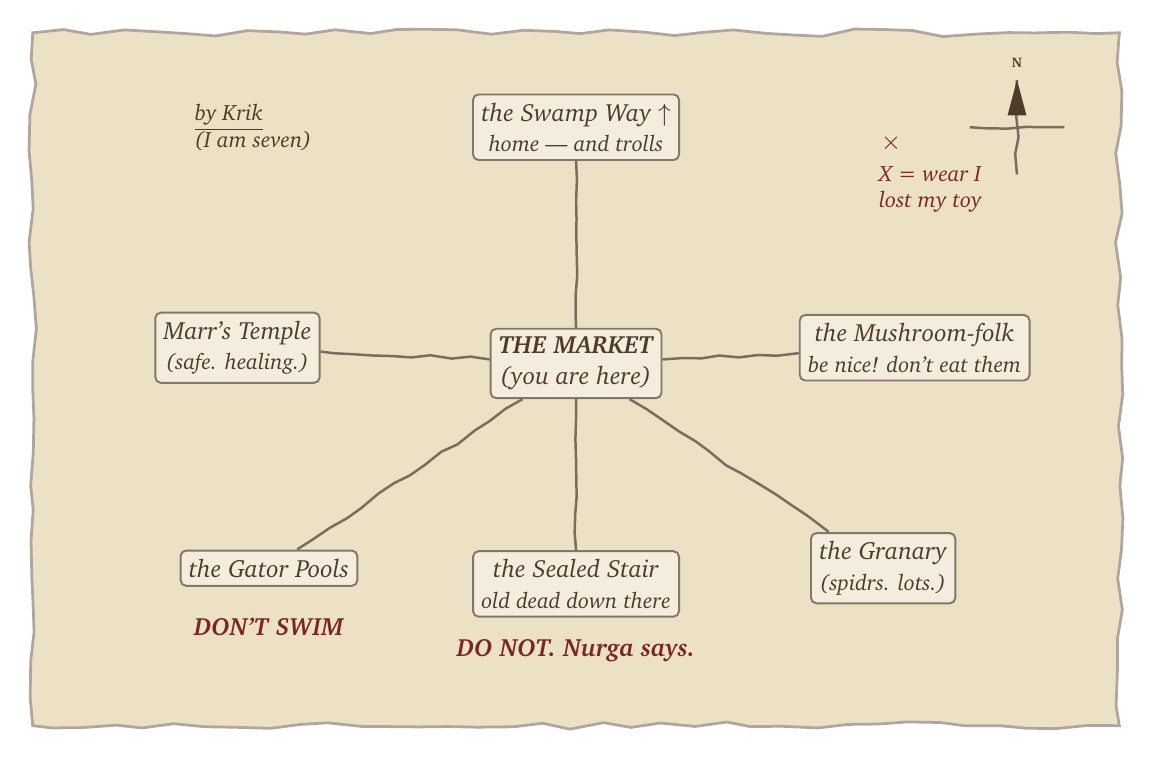
\begin{tikzpicture}[
  font=\itshape\small,
  every node/.style={text=hink},
  place/.style={draw=hink!70,line width=0.7pt,fill=hpaper!60,rounded corners=2pt,align=center,inner sep=3pt,text=hink},
  warn/.style={text=hblood,font=\itshape\bfseries\small},
  ink/.style={hink!75,line width=0.9pt,decorate,decoration={random steps,segment length=7pt,amplitude=0.7pt}}]

% torn paper
\draw[fill=hpaper,draw=hink!45,line width=1pt,decorate,
      decoration={random steps,segment length=11pt,amplitude=1.4pt}]
      (-0.4,-0.4) rectangle (13.4,8.4);

% compass
\begin{scope}[shift={(12.1,7.2)}]
  \draw[ink] (0,-0.6)--(0,0.6); \draw[ink](-0.6,0)--(0.6,0);
  \fill[hink] (0,0.6)--(-0.12,0.15)--(0.12,0.15)--cycle;
  \node[font=\tiny\bfseries] at (0,0.82){N};
\end{scope}

% nodes
\node[place] (mkt) at (6.5,4.2) {\bfseries THE MARKET\\(you are here)};
\node[place] (gate) at (6.5,7.2) {the Swamp Way $\uparrow$\\{\footnotesize home --- and trolls}};
\node[place] (temple) at (2.2,4.4) {Marr's Temple\\{\footnotesize (safe. healing.)}};
\node[place] (grotto) at (10.8,4.4) {the Mushroom-folk\\{\footnotesize be nice! don't eat them}};
\node[place] (pools) at (2.6,1.6) {the Gator Pools};
\node[warn] at (2.6,0.85) {DON'T SWIM};
\node[place] (gran) at (10.4,1.6) {the Granary\\{\footnotesize (spidrs. lots.)}};
\node[place] (stair) at (6.5,1.4) {the Sealed Stair\\{\footnotesize old dead down there}};
\node[warn] at (6.5,0.55) {DO NOT. Nurga says.};

% wobbly corridors
\draw[ink] (gate)--(mkt);
\draw[ink] (mkt)--(temple);
\draw[ink] (mkt)--(grotto);
\draw[ink] (mkt)--(pools);
\draw[ink] (mkt)--(gran);
\draw[ink] (mkt)--(stair);

% krik's scrawls
\node[warn,font=\itshape\footnotesize] at (11.0,6.6) {X = wear I};
\node[warn,font=\itshape\footnotesize] at (11.0,6.25) {lost my toy};
\node[hblood] at (10.5,7.0) {$\times$};
\node[text=hink,font=\itshape\footnotesize,align=left] at (2.4,7.2)
  {\underline{by Krik}\\ (I am seven)};
\end{tikzpicture}
\end{center}

\clearpage

\section*{Handout B --- ``The Front'' (Lower Guk)}
\emph{Copied for the party by a sergeant of the third watch from the King's own scout-maps. Everything west of the Wall is home. Everything east of it is guesswork, paid for in scouts who did not come back to correct it.}
\vspace{4pt}

\begin{center}
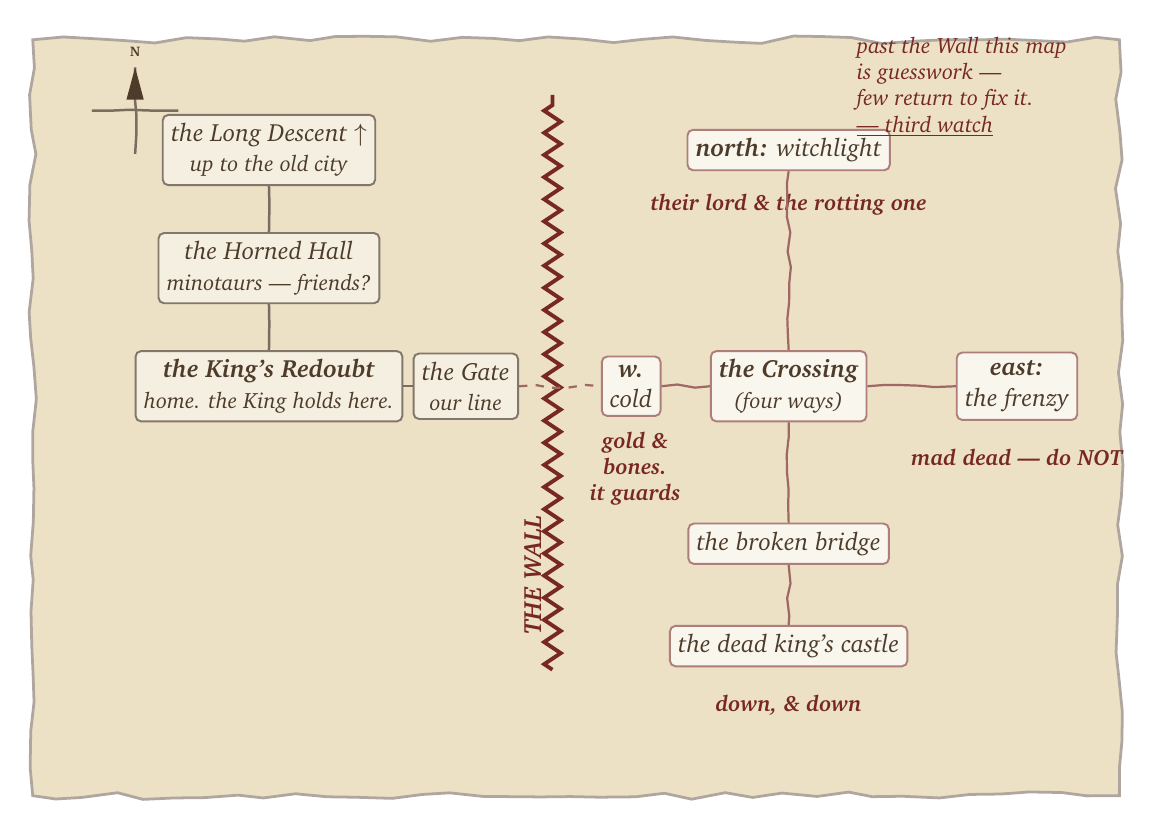
\begin{tikzpicture}[
  font=\itshape\small,
  every node/.style={text=hink},
  ours/.style={draw=hink!70,line width=0.7pt,fill=hpaper!50,rounded corners=2pt,align=center,inner sep=3pt},
  theirs/.style={draw=hblood!60,line width=0.7pt,fill=hpaper!30,rounded corners=2pt,align=center,inner sep=3pt,text=hink},
  warn/.style={text=hblood,font=\itshape\bfseries\footnotesize,align=center},
  ink/.style={hink!75,line width=0.9pt,decorate,decoration={random steps,segment length=7pt,amplitude=0.7pt}},
  redink/.style={hblood!70,line width=0.8pt,decorate,decoration={random steps,segment length=6pt,amplitude=0.8pt}}]

\draw[fill=hpaper,draw=hink!45,line width=1pt,decorate,
      decoration={random steps,segment length=11pt,amplitude=1.4pt}]
      (-0.4,-0.6) rectangle (13.4,9.0);

% compass
\begin{scope}[shift={(0.9,8.1)}]
  \draw[ink] (0,-0.55)--(0,0.55); \draw[ink](-0.55,0)--(0.55,0);
  \fill[hink] (0,0.55)--(-0.11,0.14)--(0.11,0.14)--cycle;
  \node[font=\tiny\bfseries] at (0,0.75){N};
\end{scope}

% ---- our side (west) ----
\node[ours] (descent) at (2.6,7.6) {the Long Descent $\uparrow$\\{\footnotesize up to the old city}};
\node[ours] (redoubt) at (2.6,4.6) {\bfseries the King's Redoubt\\{\footnotesize home. the King holds here.}};
\node[ours] (horn) at (2.6,6.1) {the Horned Hall\\{\footnotesize minotaurs --- friends?}};
\node[ours] (wall) at (5.1,4.6) {the Gate\\{\footnotesize our line}};

\draw[ink] (descent)--(horn); \draw[ink](horn)--(redoubt); \draw[ink](redoubt)--(wall);

% ---- THE WALL ----
\draw[hblood,line width=1.4pt,decorate,decoration={zigzag,segment length=8pt,amplitude=3pt}]
      (6.2,1.0)--(6.2,8.3);
\node[rotate=90,warn,font=\itshape\bfseries\small] at (5.95,2.2){THE WALL};

% ---- their side (east): the cross ----
\node[theirs] (cross) at (9.2,4.6) {\bfseries the Crossing\\{\footnotesize (four ways)}};
\node[theirs] (north) at (9.2,7.6) {\textbf{north:} witchlight};
\node[warn] at (9.2,6.9) {their lord \& the rotting one};
\node[theirs] (east) at (12.1,4.6) {\textbf{east:}\\the frenzy};
\node[warn] at (12.1,3.7) {mad dead --- do NOT};
\node[theirs,text=hink] (westarm) at (7.2,4.6) {\textbf{w.}\\cold};
\node[warn,align=center] at (7.25,3.55) {gold \&\\ bones.\\it guards};
\node[theirs] (bridge) at (9.2,2.6) {the broken bridge};
\node[theirs] (castle) at (9.2,1.3) {the dead king's castle};
\node[warn] at (9.2,0.55) {down, \& down};

\draw[redink] (cross)--(north);
\draw[redink] (cross)--(east);
\draw[redink] (cross)--(westarm);
\draw[redink] (cross)--(bridge); \draw[redink](bridge)--(castle);
\draw[redink,dashed] (wall)--(westarm);

% marginal warning
\node[warn,align=left,font=\itshape\footnotesize] at (11.4,8.4)
  {past the Wall this map\\ is guesswork ---\\ few return to fix it.\\ \underline{--- third watch}};
\end{tikzpicture}
\end{center}
\end{document}
